% !TEX root = ./main.tex
\chapter{Impacts of emissions spatial heterogeneity on aerosol properties and CCN activity}
%\chapter{Impacts of emissions spatial heterogeneity on aerosol properties in a particle resolved framework}

This chapter presents results for the impacts of emissions spatial heterogeneity on aerosol properties, including changes to the aerosol size distribution, composition, mixing state, and CCN activity. We begin with a set of simplified simulations to isolate the effect of spatial heterogeneity on an important aerosol process, coagulation. Subsequently, we present simulation results for full multiphase (gas and aerosol) chemistry runs and discuss changes to aerosol properties and CCN activity. We find that under high emissions spatial heterogeneity, up to 25\% more CCN activate in the upper boundary layer for supersaturations in the range $S=0.3\%$ to $S=0.6\%$. The effects of ammonium on CCN activity are also explored, as we find that high spatial heterogeneity scenarios allow more nitrate in the aerosol phase due to the avialability of free ammonia.
\section{Idealized coagulation simulations}

Prior to discussing simulations utilizing the full multiphase chemical mechanism for aerosols and chemistry, we first focus our discussion on the impact of spatial heterogeneity on aerosol number concentration due to coagulation. Coagulation is a primary mechanism for aerosol aging and its rate scales with the square of the number concentration of particles, thus making it an important aerosol process for which to evaluate the impacts of spatial heterogeneity. 

\subsection{Simulation scenarios}

\begin{figure}[h]
  \centering
    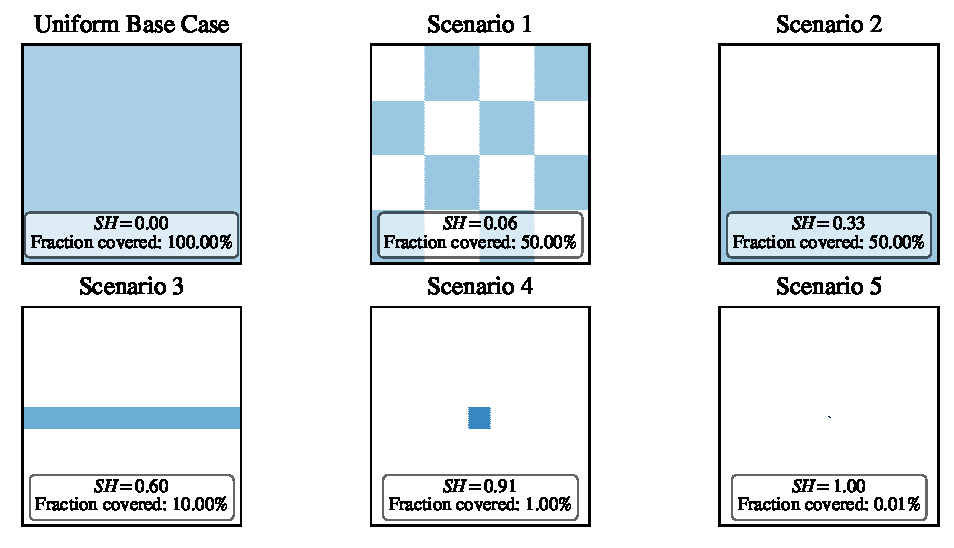
\includegraphics[width=\textwidth]{figures/chapter5/ideal-coag/ideal-coag-SH-scenarios.pdf}
    \caption{$SH$ scenarios for ideal coagulation simulations.}
    \label{fig:sh-scenarios-ideal-coag}
\end{figure}

Here we investigate the modification to the rate of coagulation under numerous spatial heterogeneity scenarios. We run a total of 6 simulations for a range of $SH$ scenarios shown in Figure \ref{fig:sh-scenarios-ideal-coag}. As with gas phase simulations in Chapter 4, the concentration of atmospheric constituents (here aerosol particle number concentration) must be scaled within the $SH$ scenario region by the ratio of the area of the uniform base case and the area occupied by the $SH$ pattern. For example, the aerosol number concentration in the central region of scenario~5 is a factor of 10,000 higher than in the uniform base case. 

Note that the setup of these simulations differs from all other simulations discussed in this thesis. Chemistry is turned off primarily for computational efficiency as, here, we are simply interested in changes to the number concentration rather than changes to aerosol composition. Instead of using initial conditions that are uniform throughout the domain, here the aerosol initial condition is set by the chosen $SH$ scenario for each vertical level in the domain (i.e., the pattern extends vertically throughout the domain). Additionally, emissions are turned off such that only coagulation is responsible for changes to aerosol number concentration.

\subsection{Results}\label{ideal-coag-results}

\begin{figure}[!h]
  \centering
    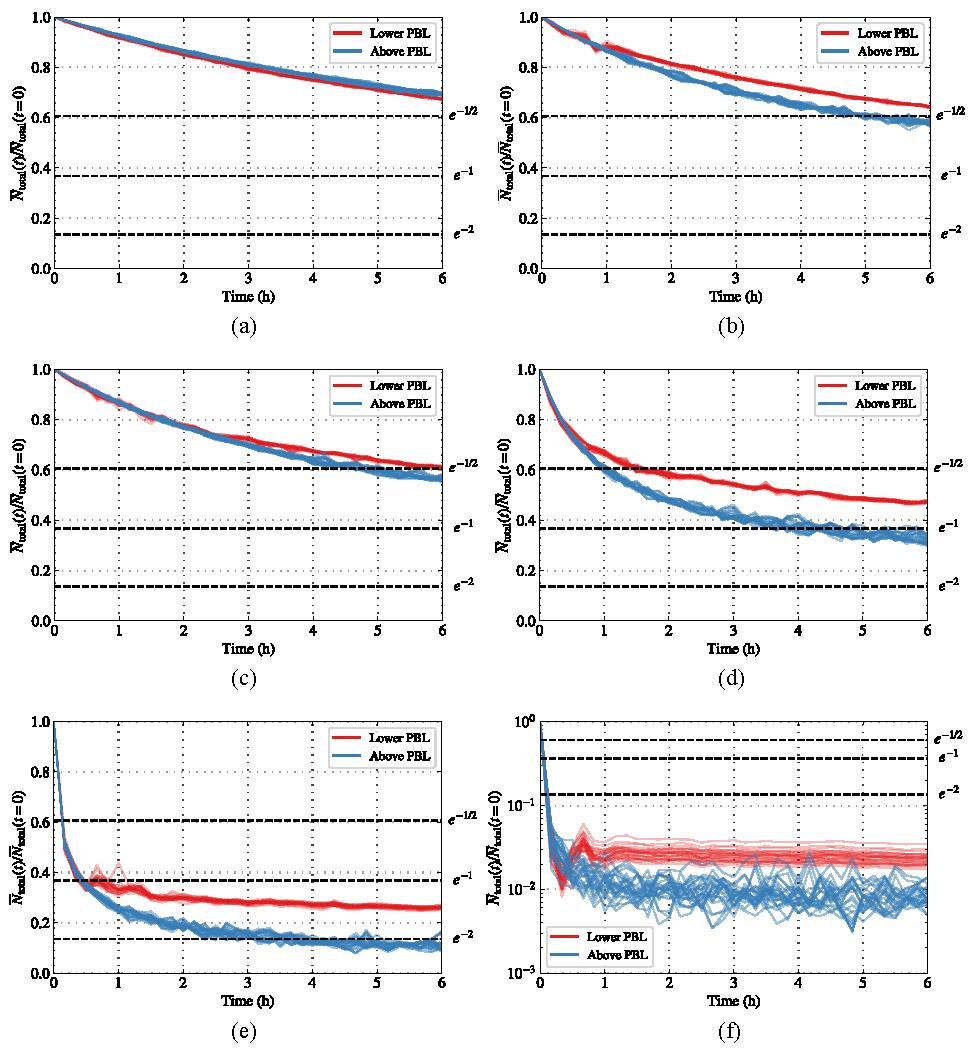
\includegraphics[width=\textwidth]{figures/chapter5/ideal-coag/NumConcTimescale_composite.pdf}
    \caption{Total number concentration for each $SH$ scenario normalized by the initial condition total number concentration. Lines indicate normalized number concentration averaged over each vertical level in the domain. (a) Uniform base case. (b--f) Scenarios 1--5}
    \label{fig:numconc-timescales}
\end{figure}

Figure \ref{fig:numconc-timescales} show how the total number concentration of aerosol particles decreases due to coagulation under each $SH$ scenario. For each scenario, we compute the average number concentration at each vertical level and time $t$, $\overline{N}_{\text{total}}(t)$. This number concentration is then normalized by the number concentration at time $t=0$, $\overline{N}_{\text{total}}(t=0)$. A subset of number concentration timeseries are shown in Figure \ref{fig:numconc-timescales} for the lowest 20 vertical levels of the planetary boundary layer ($z=0$ m to $z\approx200$ m) and highest 20 vertical levels in the domain above the planetary boundary layer ($z\approx1.8$ km to $z=2$ km). The reason for this grouping is that these two regions are notably different in terms of the rate at which the total number concentration decreases. For scenarios 1--5 (Figure \ref{fig:numconc-timescales} subfigures b--f), we find that the total number concentration decreases slower in the lower planetary boundary layer than above the planetary boundary layer. A notable exception to this trend is the uniform base case (Figure \ref{fig:numconc-timescales} subfigure a). Recall that the rate of coagulation scales as the square of the number of particles. As a result, highly heterogeneous patterns that require significant scaling up of the number concentration will have greater rates of coagulation within the high-concentration region associated with the $SH$ pattern. As the planetary boundary layer develops and turbulent motion begins to diffuse the initial structure of the $SH$ pattern, concentration gradients are reduced, resulting in a reduction of the rate of coagulation. This turbulent motion does not disturb the structure of the $SH$ pattern above the planetary boundary layer, and thus coagulation will proceed at a faster rate within the high concentration region of the $SH$ pattern.

We find that as the $SH$ increases across scenarios, the total number concentration is reduced more rapidly. For each plot in Figure \ref{fig:numconc-timescales}, we include horizontal dashed lines indicating the e-folding time alongside a half e-folding time ($e^{-1/2}$) and double e-folding time as the rate at which the total number concentration is reduced under $SH$ scenarios varies widely.  

\begin{figure}[!t]
  \centering
    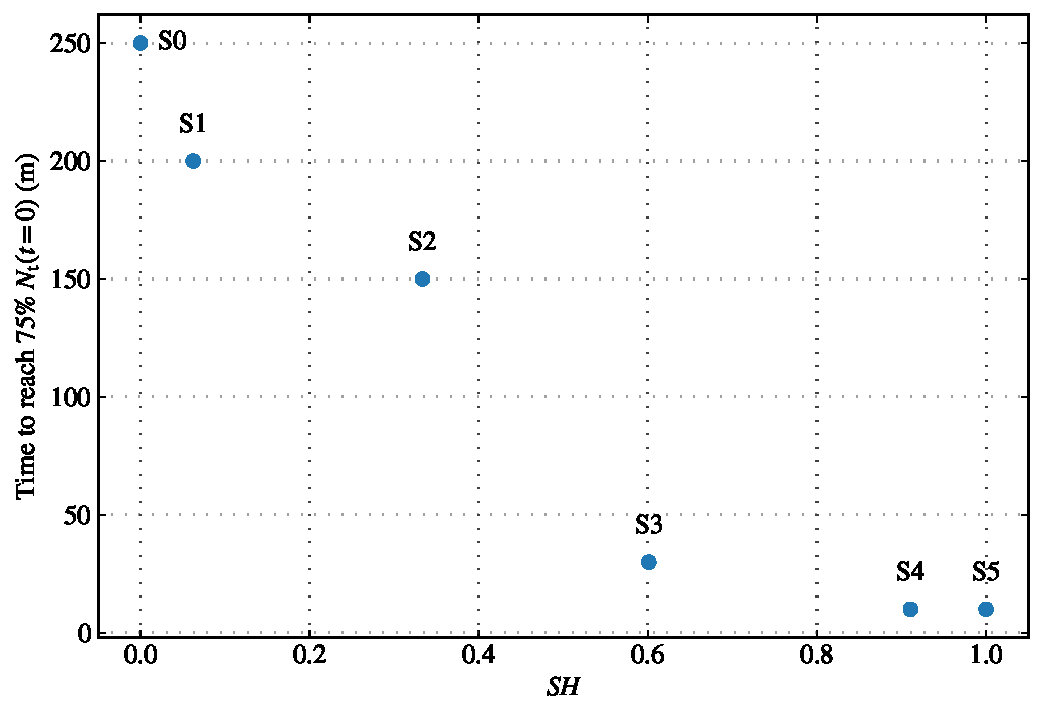
\includegraphics[width=.8\textwidth]{figures/chapter5/ideal-coag/TimeTo75pcnt_vs_SH.pdf}
    \caption{Time required in minutes for the total number concentration in the lowest 200 m of the planetary boundary layer to be reduced to 75\% of the initial value vs. scenario~$SH$. ``S0" is the uniform base case, with all other scenarios labeled S1--S5.}
    \label{fig:numconc-timescales-to-75pcent}
\end{figure}

Figure \ref{fig:numconc-timescales-to-75pcent} shows the time required the number concentration in the lower planetary boundary layer to be reduced to 75\% of the initial total number concentration plotted against the spatial heterogeneity of each scenario. The uniform base case (``S0") requires over four hours to reach 75\% of the initial total concentration, while the highest heterogeneity scenarios 4 and 5 require only 10 minutes.

% --------------------------------------------
\section{Full multiphase simulations}

Here we discuss simulations containing full multiphase chemistry under numerous emissions spatial heterogeneity scenarios. A summary of emissions scenarios is presented followed by presentation of results pertaining to the aerosol state and properties under each emission scenario. 

\subsection{Simulated emissions scenarios}

\begin{figure}[t]
  \centering
    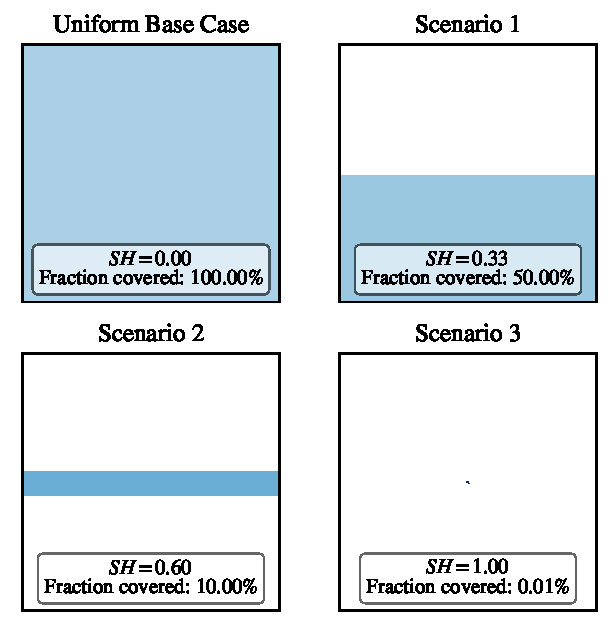
\includegraphics[width=.6\textwidth]{figures/SH-scenarios-main-runs.pdf}
    \caption{Emissions scenarios for multiphase chemistry simulations. The spatial heterogeneity of each emission scenario is listed in the lower portion of each scenario alongside domain mean and variance.
}
    \label{fig:aerosol-emission-scenarios}
\end{figure}

Scenarios discussed in this section match the set of emissions scenarios presented in Chapter 4 Section \ref{gas-emission-scenarios}. We evaluate changes to the aerosol population under four scenarios with increasing spatial heterogeneity as shown in Figure \ref{fig:aerosol-emission-scenarios}. As with previous results, the first scenario is a ``uniform base case", characterized by diffuse and uniform emissions across the ground level of the domain ($SH=0$). Scenarios 1--3 present progressively higher heterogeneity up to $SH=1$, whereby the rate of emissions is scaled to ensure the total mass per unit time emitted across each scenario is the same.

As a reminder to the reader, initial conditions and emissions for the gas phase and aerosol are discussed in Chapter 3 Section \ref{gas-phase-ics-and-emiss} and Section \ref{aerosol-ics-and-emiss}, respectively. 

\subsection{Aerosol size distributions}

\begin{figure}[!t]
  \centering
    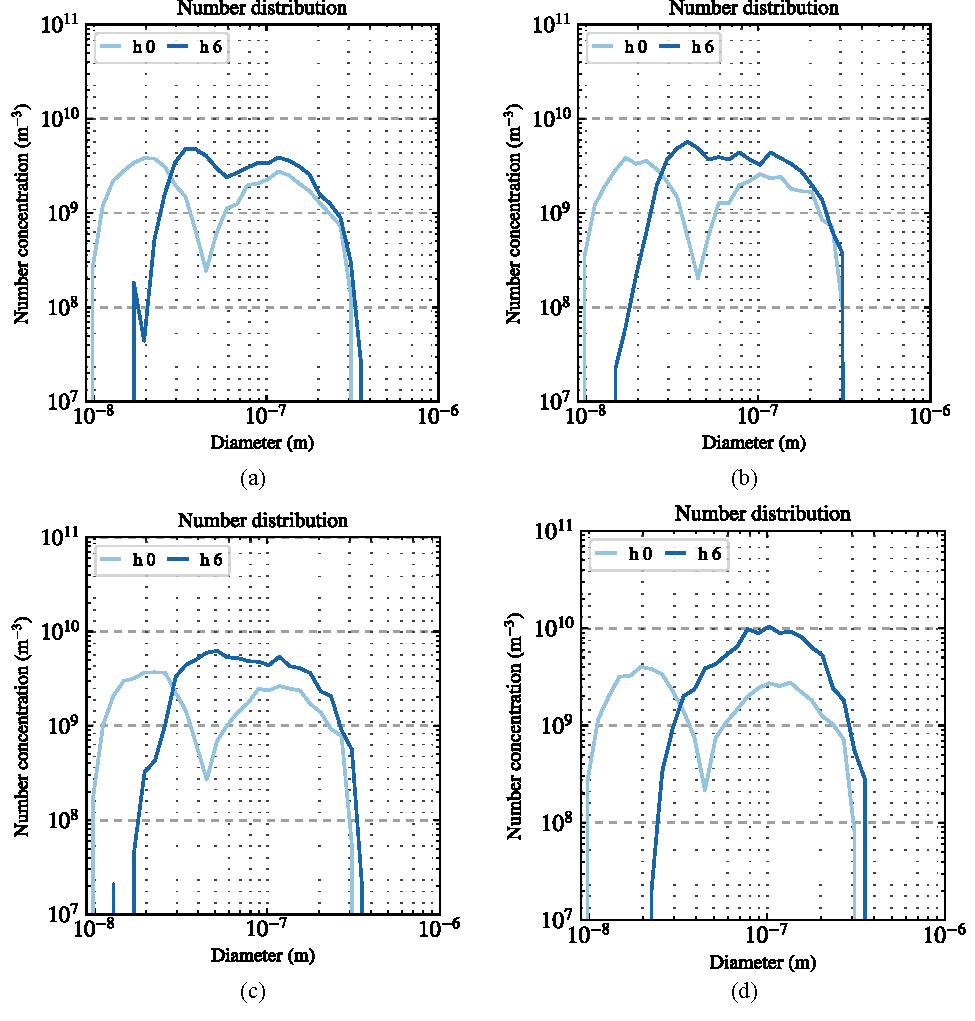
\includegraphics[width=\textwidth]{figures/chapter5/number-distribution-plots.pdf}
    \caption{Aerosol number distribution plots for each emissions scenario. The distribution initial condition (light blue) is shown alongside the distribution at the end of each simulation ($t=6$ h).}
    \label{fig:number-dists}
\end{figure}

Figure \ref{fig:number-dists} shows aerosol number distributions for each simulated emissions scenario. The initial condition size distribution is presented alongside the size distribution at the end of each simulation ($t=6$ h). Each size distribution is taken from a vertical level in the upper boundary layer at $z\approx800$ \si{m}. Due to the stochastic treatment of aerosols in the WRF-PartMC model and the chosen number of computational particles per grid cell ($n=100$), size distributions represent the average distribution in a 1 \si{km^2} region centered over the emissions plume. For all scenarios except scenario~1, this region is located at the center of the domain. For scenario~1, emissions are released in one half of the domain that is offset from the center, thus the averaging region for the size distribution is located in the center of the emissions patch. WRF-PartMC returns the number distribution in 100 logarithmically spaced bins ranging from $10^{-9}$ m to $10^{-3}$ m.

For each scenario displayed in Figure \ref{fig:number-dists}, the initial condition size distribution is shown in light blue. The distribution is bimodal, containing an Aitken (left) and accumulation mode (right). The Aitken mode contains fine particulates and is centered around $20$ nm, while the accumulation mode contains slightly fewer particles and is centered around 116 nm. 

After 6 hours, the number of particles with diameter smaller than $\approx30$ nm is significantly reduced as these small particles undergo coagulation and growth by gas-to-particle partitioning. For particle diameters greater than $\approx30$ nm, the number concentration is increased under each scenario as primary aerosol are emitted and particles undergo aging. For the uniform base case (Figure \ref{fig:number-dists} subplot a), the distribution still takes on a bimodal shape at $t=6$ h, however the Aitken mode has been replaced by a mode centered around 35 nm and is likely a combination of primary aerosol emissions and growth of smaller particles from the initial Aitken mode. 

Moving to higher emissions spatial heterogeneity scenarios, we find that the number distribution loses its bimodal shape after 6 hours, especially under the highest heterogeneity scenario, scenario~3 (Figure \ref{fig:number-dists} subplot d). For scenario~3, the number distribution peaks around 0.1 $\mu$m. Compared with the uniform base case, the number concentration of particles in the accumulation mode near $D_p = 0.1$ \si{\mu m} is approximately half an order of magnitude higher ($10^{10}$ \si{m^{-3}} vs. $4\cdot10^9$ \si{m^{-3}}).

\begin{figure}[!t]
  \centering
    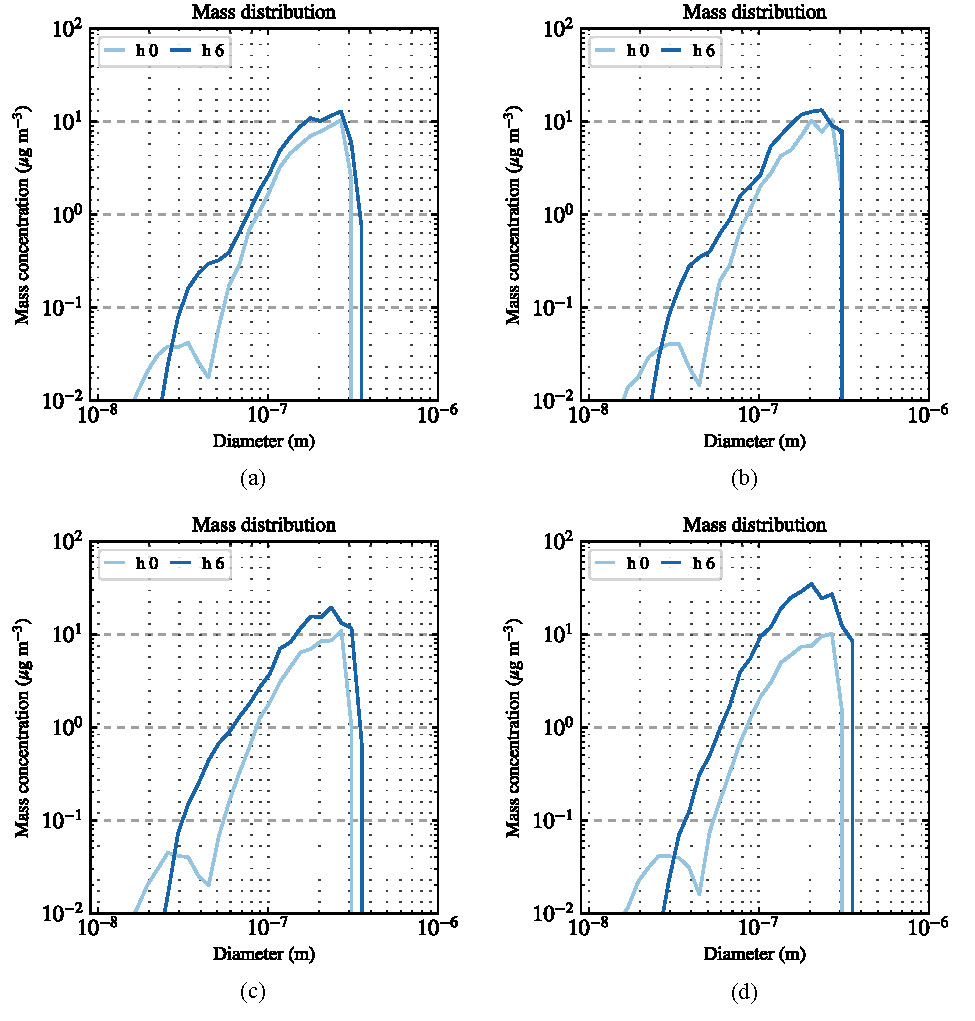
\includegraphics[width=\textwidth]{figures/chapter5/mass-distribution-plots.pdf}
    \caption{Aerosol mass distribution plots for each emissions scenario. The distribution initial condition (light blue) is shown alongside the distribution at the end of each simulation ($t=6$ h).}
    \label{fig:mass-dists}
\end{figure}

Figure \ref{fig:mass-dists} shows mass distribution plots for each emissions scenario. Mass distributions were taken from the same upper boundary layer region as number distributions and the same averaging technique was applied over a 1 \si{km^2} region centered over the emissions plume. Mass concentrations are presented in \si{\mu g.m^{-3}}. 

The mass distribution initial condition presents a bimodal profile as before; however, much more mass is concentrated in the larger accumulation mode particles due to the cubic scaling between mass and particle diameter, $M_p \propto D_p^3$. After six hours, the mass concentration of all particles with diameters larger than $\approx25$ nm is increased. The distribution for the uniform base case contains two distinct modes, one corresponding to the accumulation mode and an additional mode centered around $30$ nm. This mode contains both primary aerosol and aged aerosol due to gas-particle partitioning and coagulation of Aitken mode particles. 

As with the number distributions, when moving from low to high $SH$ scenarios, the bimodal shape of the mass distribution is replaced by a single mode centered around the accumulation mode, peaking at $D_p = 0.2$ \si{\mu m}. When compared to the uniform base case, mass concentrations in the accumulation mode for the highest $SH$ case, scenario~3, are approximately 3 times higher ($\approx30$ \si{\mu g.m^{-3}} vs. $\approx10$ \si{\mu g.m^{-3}}).


\subsection{Aerosol composition}

\begin{figure}[!t]
  \centering
    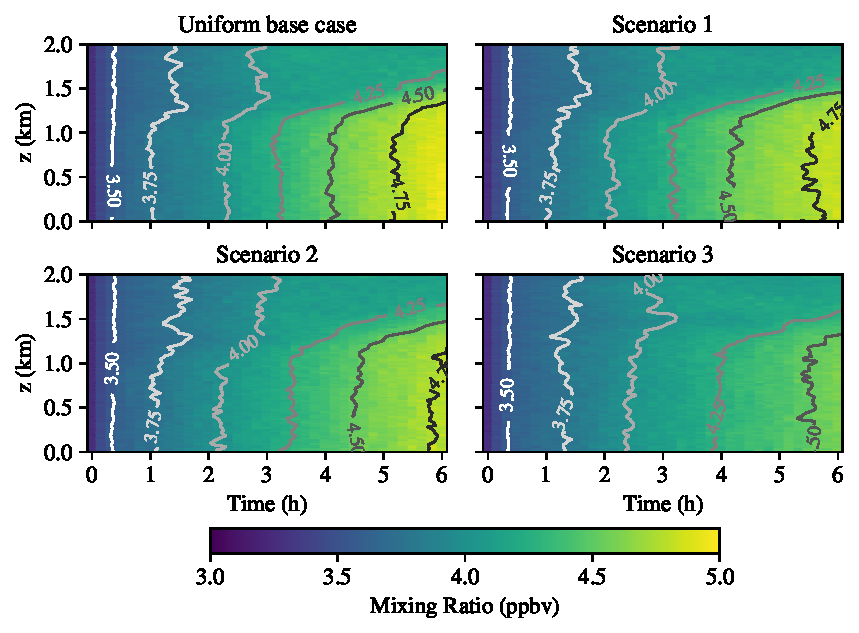
\includegraphics[width=\textwidth]{figures/chapter5/height-time-pmc_SO4-four-scenarios.pdf}
    \caption{Time-height plots for aerosol sulfate across each emissions scenario. Isopleths indicate sulfate mixing ratio in ppbv ranging from 3.5--4.75 ppbv.}
    \label{fig:ht-so4}
\end{figure}

Figure \ref{fig:ht-so4} shows time-height plots for aerosol sulfate concentrations in parts per billion by volume (ppbv). Mixing ratios are shown instead of mass concentrations as mixing ratio is independent of the atmospheric pressure and density. To compute the mixing ratio in ppbv for aerosol concentrations natively output by WRF-PartMC in \si{kg.m^{-3}}, concentrations are multiplied by the inverse of atmospheric density for each vertical level and by a factor of $10^9$ to convert from mol/mol to parts per billion.

As with previous time-height plots presented in Chapter 4, each pixel in the time-height grid mesh represents the average concentration over a given vertical level and time. Isopleths indicate lines of constant sulfate mixing ratios, ranging from 3.50 to 4.75 ppbv in increments of 0.25 ppbv.

Initially, each scenario contains a uniform sulfate concentration of $\approx3.5$ ppbv. During the first hour, concentrations gradually increase everywhere, likely due to the oxidation of ambient SO$_2$ and partitioning of resulting H$_2$SO$_4$ into the aerosol phase due to its extremely low volatility vapor pressure. As emissions turn on at $t=1$ h, the concentration of sulfate across emissions scenarios begins to diverge. In the uniform base case, sulfate concentrations steadily increase within the planetary boundary layer through $t=6$ h up to 4.75 ppbv. For high $SH$ scenarios such as scenario~3, the rate of increase in sulfate concentrations is suppressed--it takes nearly two hours for sulfate concentrations to increase from 4.25 ppbv at $t=4$ h to 4.50 by $t=6$ h whereas the same increase under the uniform base case takes approximately 1 hour between $t=3$ h and $t=4$ h. This results in lower sulfate concentrations within the planetary boundary layer under high $SH$ scenarios through $t=6$ h. For each scenario and timestep, we find that sulfate concentrations are approximately uniform throughout the planetary boundary layer. This is to be expected, as the vapor pressure of H$_2$SO$_4$ is only a weak function of temperature over the range of temperatures represented in the simulated planetary boundary layer ($\approx303$ K near the surface decreasing to $\approx293$ K at top of the planetary boundary layer).

\begin{figure}[!t]
  \centering
    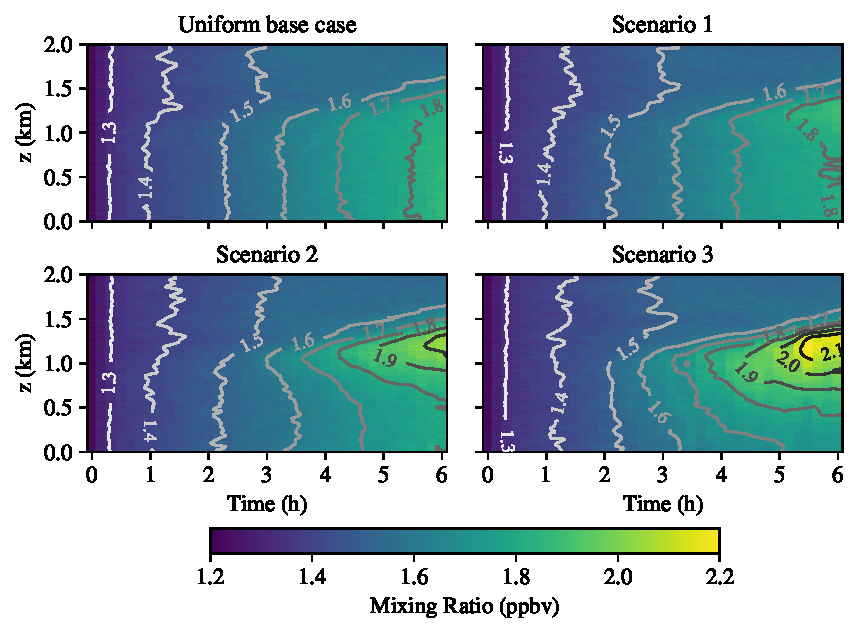
\includegraphics[width=\textwidth]{figures/chapter5/height-time-pmc_NH4-four-scenarios.pdf}
    \caption{Time-height plots for aerosol ammonium across each emissions scenario. Isopleths indicate ammonium mixing ratio in ppbv ranging from 1.3--2.1 ppbv.}
    \label{fig:ht-nh4}
\end{figure}

Time-height plots for ammonium concentrations in each emissions scenario are shown in Figure \ref{fig:ht-nh4}. Initially, aerosol ammonium concentrations are uniformly 1.2 ppbv everywhere. Ammonium concentrations steadily increase as ambient ammonia partitions into the aerosol phase. Following the release of emissions at $t=1$ h, ammonium concentrations are similar across each scenario between $t=1$ h to $t=2$ h with concentrations increasing to 1.5 ppbv. Subsequently, ammonium concentrations differ both spatially and temporally across emissions scenarios. Ammonium concentrations in the base case remain diffuse and relatively uniform throughout the planetary boundary layer, increasing to 1.8 ppbv through $t=6$ h. As $SH$ increases across scenarios, ammonium concentrations in the upper planetary boundary layer increase to as much as 2.1 ppbv in scenario~3 by $t=5$ to $t=6$ h. Meanwhile, concentrations in the lower planetary boundary layer remain near 1.7--1.8 ppbv.

\begin{figure}[!t]
  \centering
    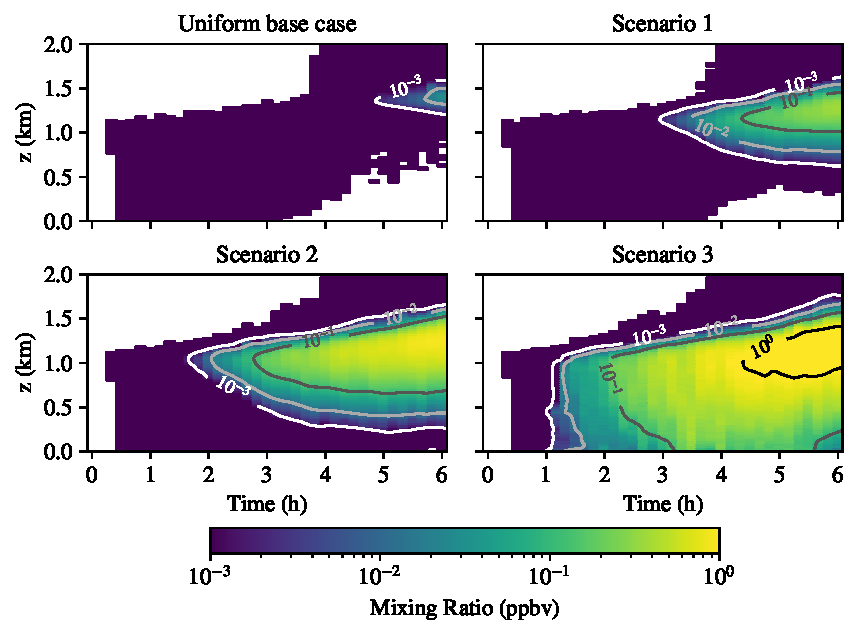
\includegraphics[width=\textwidth]{figures/chapter5/height-time-pmc_NO3-four-scenarios.pdf}
    \caption{Time-height plots for aerosol nitrate across each emissions scenario. Isopleths indicate nitrate mixing ratio in ppbv ranging from $10^{-3}$ to $10^0$ ppbv.}
    \label{fig:ht-no3}
\end{figure}

Figure \ref{fig:ht-no3} shows time-height plots of aerosol nitrate concentrations for each emissions scenario. Note the logarithmic scaling for the color bar as nitrate concentrations span numerous orders of magnitude due to trace concentrations in some regions. Initially, no nitrate is present in the aerosol phase (zero concentrations are indicated by white). Nitrate concentrations remain at or below $10^{-3}$ ppbv in the free troposphere throughout each scenario. When compared to sulfate and ammonium, the abundance of nitrate is most sensitive to emissions spatial heterogeneity as only trace amounts of nitrate ($10^{-3}$--$10^{-2}$ ppbv) are present in the upper planetary boundary layer in the uniform base case, whereas concentrations reach 1 ppbv in the upper planetary boundary layer in scenario~3. Additionally, the formation of nitrate occurs over a broader depth of the planetary boundary layer for high $SH$ scenarios and the onset of formation occurs earlier.

Both ammonium and nitrate increase in concentration with height in the planetary boundary layer due to the strong dependence of ammonium nitrate formation on temperature. Over the range of ambient temperatures observed in the boundary layer, the equilibrium dissociation constant of ammonium nitrate varies over several orders of magnitude and increases with temperature. This means that at lower temperatures conditions such as the upper planetary boundary layer, the equilibrium of ammonia and nitric acid in the gas phase will be low and the formation of ammonium nitrate in the aerosol phase is preferred. 

%\hl{Seinfeld and Pandis (10.4.4) discuss the SNA system and the two important regimes, ammonia-rich and ammonia-poor. In ammonia-poor, there isnt enough ammonia to neutralize the sulfate and most ammonia will exist in the gas phase and consequentially ammonium nitrate levels will also be low. In the ammonia rich case, there is excess ammonium than what is necessary to neutral all of the sulfate and thus the free ammonia will form ammonium nitrate.}

\begin{figure}[!t]
  \centering
    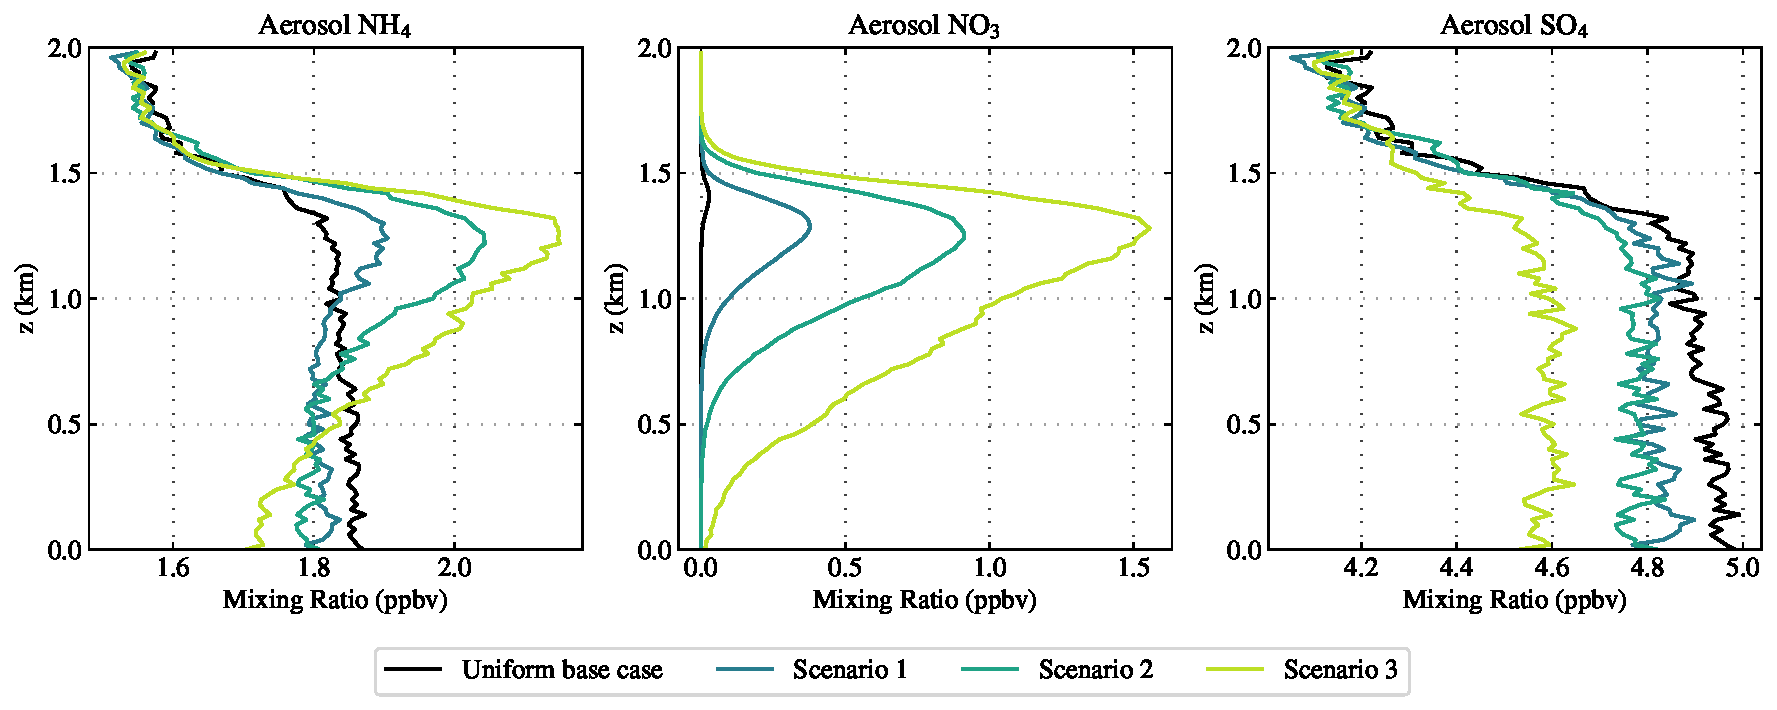
\includegraphics[width=\textwidth]{figures/chapter5/aerosol-SNA-vertical-profiles-time36.pdf}
    \caption{Vertical profiles of aerosol ammonia, nitrate, and sulfate at $t=6$ h.}
    \label{fig:sna-vertical-profile}
\end{figure}

Time-height plots for sulfate, ammonium, and nitrate capture the spatial and temporal variation of each aerosol species across each emissions scenario. However, to help quantitatively summarize and compare the relative abundances of each species, we focus here on the final state of the sulfate-nitrate-ammonium system at the end of each simulation, $t=6$ h. Figure \ref{fig:sna-vertical-profile} shows vertical profiles of ammonia, nitrate, and sulfate for $t=6$ h, whereby each vertical profile represents the horizontally averaged concentration in ppbv at each vertical level of the domain.

We find that ammonium has a relatively uniform concentration of 1.85 ppbv in the planetary boundary layer for the uniform base case. As the spatial heterogeneity of emissions scenarios increases, the abundance of ammonium increases towards the upper planetary boundary layer (which reaches a height of $z\approx1.5$ km by $t=6$ h), reaching 2.1 ppbv in the highest $SH$ scenario. Near the surface, ammonia concentrations decrease as the $SH$ of the emissions scenario increases. 

Nitrate levels increase with increasing emissions $SH$. For lower $SH$ scenarios, this increase is localized to the upper planetary boundary layer. As emissions $SH$ increases across scenarios, nitrate concentrations also increase in the lower planetary boundary layer, however the region of highest nitrate concentrations remains vertically distributed in the upper planetary boundary layer. Nitrate levels reach up to 1.5 ppbv at $z\approx1.25$ km in the highest $SH$ scenario.  

Compared with ammonium and nitrate, sulfate concentrations within the planetary boundary layer are more vertically uniform for each emissions scenario. As the $SH$ of emissions scenarios increases, sulfate concentrations are reduced by approximately the same amount everywhere in the planetary boundary layer from a planetary boundary layer average of 4.9 ppbv in the uniform base case to 4.6 ppbv in scenario~3. 

\begin{figure}[!t]
  \centering
    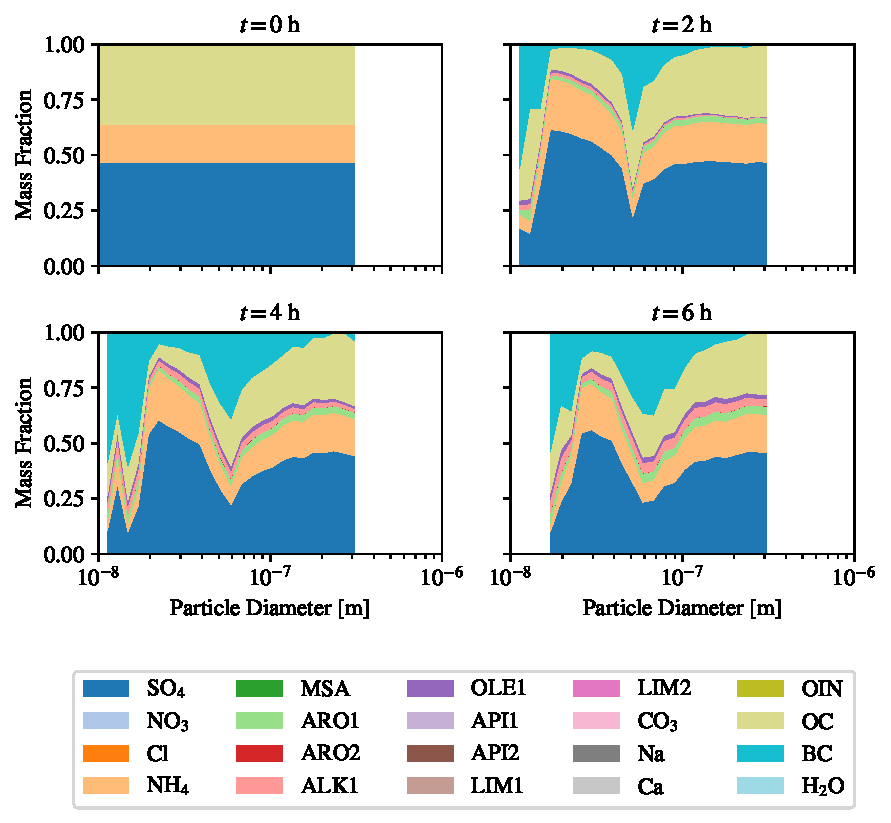
\includegraphics[width=\textwidth]{figures/chapter5/speciated-mass-frac-four-panel-uniform-basecase-z40.pdf}
    \caption{Size-resolved mass fraction for the uniform base case at regular 2-hour intervals.}
    \label{fig:mass-frac-ub}
\end{figure}

Figure \ref{fig:mass-frac-ub} shows the size-resolved mass fraction of aerosol particles in the upper planetary boundary layer ($z\approx800$ m) at 2-hour intervals for the uniform base case. The average of species mass as a fraction of aerosol total mass is displayed for each aerosol species in WRF-PartMC. As with number and mass distribution plots, species concentrations are size-resolved with 100 logarithmically spaced bins between $10^{-9}$ and $10^{-3}$ m. Mass fractions are computed by dividing the mass of each species by the total mass of a bin. In order to reduce stochastic noise, an averaging strategy similar to that utilized for the number and mass distribution plots is employed, whereby mass fractions are computed for aerosol particles contained within a 1 \si{km^2} cross section of the domain centered over the emissions plume. Aerosol species model symbols are included in the key of Figure \ref{fig:mass-frac-ub}. A comprehensive list of aerosol species in WRF-PartMC is contained in Table \ref{table:wrf-partmc-species} alongside a description of each species model symbol". 

\begin{table}[!t]
\centering
\caption{Aerosol species and associated hygroscopicities in WRF-PartMC}
\begin{tabular*}{.6\linewidth}{@{\extracolsep{\fill}} lcc}
\\[-2ex]\hline 
     \hline \\[-2ex] \textbf{Aerosol species} & \textbf{Model symbol} & \textbf{Hygroscopicity $\kappa$} \\
\midrule
Sulfate & SO4 & 0.65 \\
Nitrate & NO3 & 0.65 \\
Chloride & Cl & 0.53 \\
Ammonium & NH4 & 0.65 \\
Nethanesulfonic acid & MSA & 0.53 \\
Aromatic & ARO1 & 0.1 \\
Aromatic & ARO2 & 0.1 \\
Alkanes & ALK1 & 0.1 \\
Olefin & OLE1 & 0.1 \\
$\alpha$-pinene & API1 & 0.1 \\
$\alpha$-pinene & API2 & 0.1 \\
Limonene & LIM1 & 0.1 \\
Limonene & LIM2 & 0.1 \\
Carbonate & CO3 & 0.53 \\
Sodium & Na & 0.53 \\
Calcium & Ca & 0.53 \\
Other inorganics & OIN & 0.1 \\
Organic carbon & OC & 0.001 \\
Black carbon & BC & 0 \\
Water & H2O & 0 \\
\\[-2ex]\hline 
     \hline \\[-2ex]
\end{tabular*}
\label{table:wrf-partmc-species}
\end{table}

For the initial condition, the composition of all particles is identical, with a mixture comprised of sulfate, organic carbon (OC), and ammonium. Once emissions are active at $t=1$ h, the release of carbonaceous primary aerosol introduces black carbon (BC) into the aerosol population.  By $t=6$ h, BC makes up a meaningful fraction of aerosol mass for fine particulates; particles with diameter $\approx20$ nm are up to 50\% BC and particles near 50--60 nm are $\approx40\%$ BC.

Additionally, volatile organic compounds (VOCs) are emitted in the gas phase which are oxidized, lowering their volatility and allowing them to condense into the aerosol phase as secondary organic aerosol (SOA). SOA species are organized by functional group in WRF-PartMC and include aromatics (``ARO1", ``ARO2"), alkanes (``ALK1", ``ALK2"), limonenes (``LIM1", ``LIM2"), etc (see Table \ref{table:wrf-partmc-species} for a full list). In size-resolved mass fraction plots, SOA appears as a ribbon of green, pink, and purple atop nitrate (orange), indicating that alkanes, olefins, and aromatics comprise the bulk of SOA species present in aerosol particles. In total, SOA makes up a small fraction of aerosol mass, reaching up to 10\% of total mass by $t=6$ h.

Throughout the uniform base case simulation, the mass fraction of sulfate makes up a large portion of aerosol mass. After initially being comprised of 45\% sulfate across all aerosol diameters, by $t=6$ h, sulfate mass fraction varies between a minimum of 10\% for ultrafine particles less than 20 nm and peaks at $\approx50\%$ for particles near 30 nm. Particles in the accumulation mode are comprised of 30--40\% sulfate. Ammonium initially comprises $\approx10\%$ of aerosol mass fraction and its relative contribution to total aerosol mass is fairly consistent across time, especially for larger particles ($D_p > 0.1$ \si{\mu m}). The mass fraction of ammonium reaches a minimum for particles ultrafine particles less than 30 nm in diameter. It is important to note that no nitrate is present at any point during the uniform base case simulation.

\begin{figure}[!t]
  \centering
    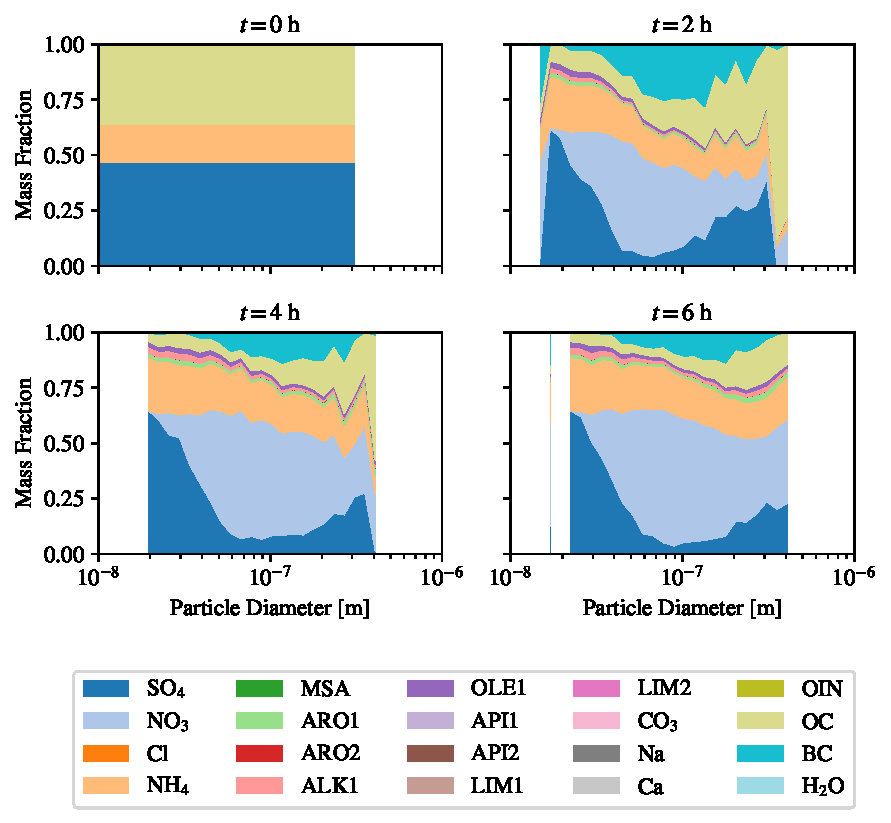
\includegraphics[width=\textwidth]{figures/chapter5/speciated-mass-frac-four-panel-point-source-1x1-z40.pdf}
    \caption{Size-resolved mass fraction for emissions scenario~3 at regular 2-hour intervals showing species mass fraction as a percent of total aerosol mass vs. particle diameter.}
    \label{fig:mass-frac-s3}
\end{figure}

Figure \ref{fig:mass-frac-s3} shows size-resolved mass fraction plots for the highest heterogeneity case, scenario~3. By $t=6$ h, the composition of aerosol particles is markedly different than in the uniform base case shown in Figure \ref{fig:mass-frac-ub}. Most notably, we find that nitrate comprises a large fraction of aerosol mass, especially for particle diameters near $D_p\approx0.1$ \si{\mu m}. As particle diameter decreases below 0.1 \si{\mu m}, the mass fraction of sulfate steady increases from less than 10\% to nearly 60\% for particles with diameter $D_p  \lesssim 30$ nm. Sulfate and nitrate effectively replace the large mass fraction of BC found for these ultrafine particles. By $t=6$ h, sulfate, nitrate, and ammonium jointly comprise a majority of aerosol mass across all particles diameters observed in emissions scenario~3. For particles smaller than 0.1 \si{\mu m}, sulfate, nitrate, and ammonium represent over 80\% of aerosol mass. For particles larger than 0.1 \si{\mu m}, these species comprise 70--80\% of aerosol mass.

Differences observed in aerosol composition are important due to the varying properties of aerosol species and their downstream influence on the atmospheric state. For example, particle hygroscopicity determines the critical supersaturation at which a particle of a given diameter will active as a cloud condensation nucleus. Hygroscopicity is parameterized using the $\kappa$-Köhler theory of \textcite{petters_single_2007}. $\kappa$-Köhler theory is a modification to Köhler's relationship for determining the saturation ratio over a particle and the critical supersaturation at which the particle activates \parencite{kohler_nucleus_1936}. Each aerosol species has an associated hygroscopicity $\kappa$, and the total particle $\kappa$ is a volume-weighted sum of each species $\kappa$. Note that Table \ref{table:wrf-partmc-species} lists the hygroscopicity parameter $\kappa$ of each aerosol species and is highly variable (e.g., the hygroscopicity of BC is zero while sulfate has a hygroscopicity of 0.65). Values of  $\kappa$ greater than 0.5 indicate the aerosol species has a high hygroscopicity, while $\kappa=0$ corresponds to a nonhygroscopic compound.

\begin{figure}[!t]
  \centering
    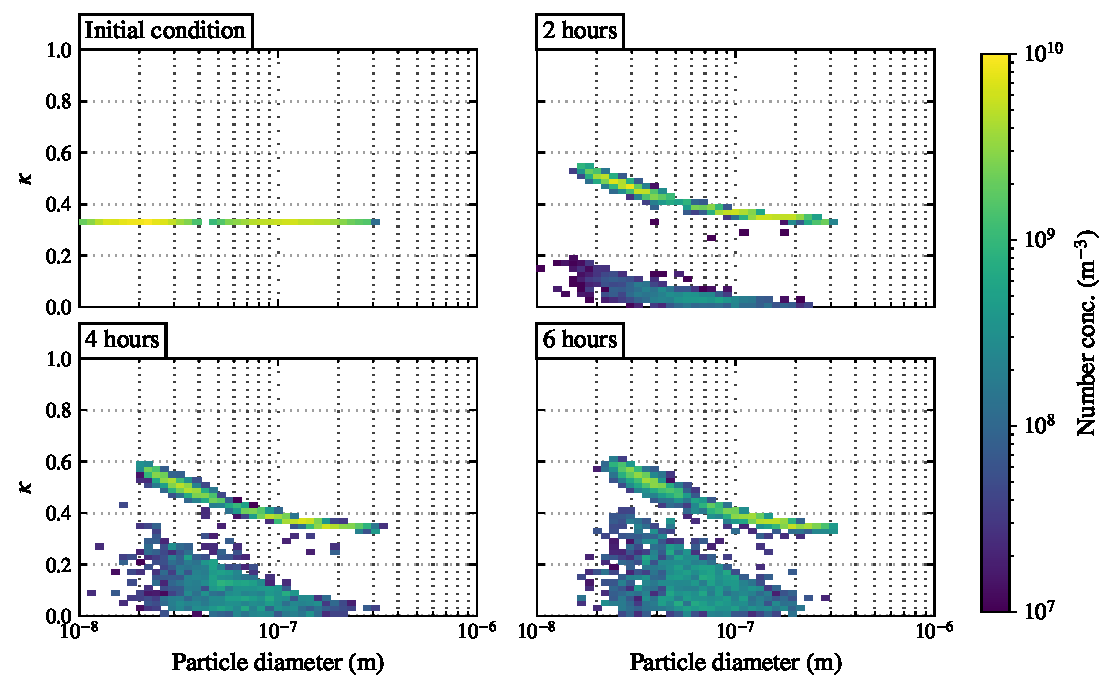
\includegraphics[width=\textwidth]{figures/chapter5/2d-kappa-dist-4-panel-uniform-basecase-z40.pdf}
    \caption{2-dimensional number distributions $n(D_p, \kappa)$ at regular two-hour intervals for the uniform base case.}
    \label{fig:2d-kappa-dist-ub}
\end{figure}

Figure \ref{fig:2d-kappa-dist-ub} shows two-dimensional number distributions at regular two hour intervals for the uniform base case in the upper planetary boundary layer ($z\approx800$ m). The x-axis indicates particle diameter in meters, while hygroscopicity $\kappa$ is plotted along the y-axis. Particles are binned into a two-dimensional histogram by diameter (50 bins from 10 nm to 1 $\mu$m) and $\kappa$ (50 bins from 0 to 1) and the number concentration within each bin is tallied and displayed as a colorbar. Bins with zero particles are filled in white.

At the initial condition, we find that all particles posses the same total hygroscopicity, $\kappa=0.32$, as each is a mixture of ammonium sulfate and OC. Beginning at $t=1$ h, emissions of primary aerosol and gas phase species alter the distribution of particle hygroscopicity. Recall that emitted primary aerosol are composed of OC and BC with $\kappa$ values 0.001 and 0, respectively. This results in a distribution of low-$\kappa$ aerosol particles situated beneath the sulfate-rich aerosol. As the simulation evolves, gas-particle partitioning and coagulation age the aerosol population, increasing particle hygroscopicity.

\begin{figure}[!t]
  \centering
    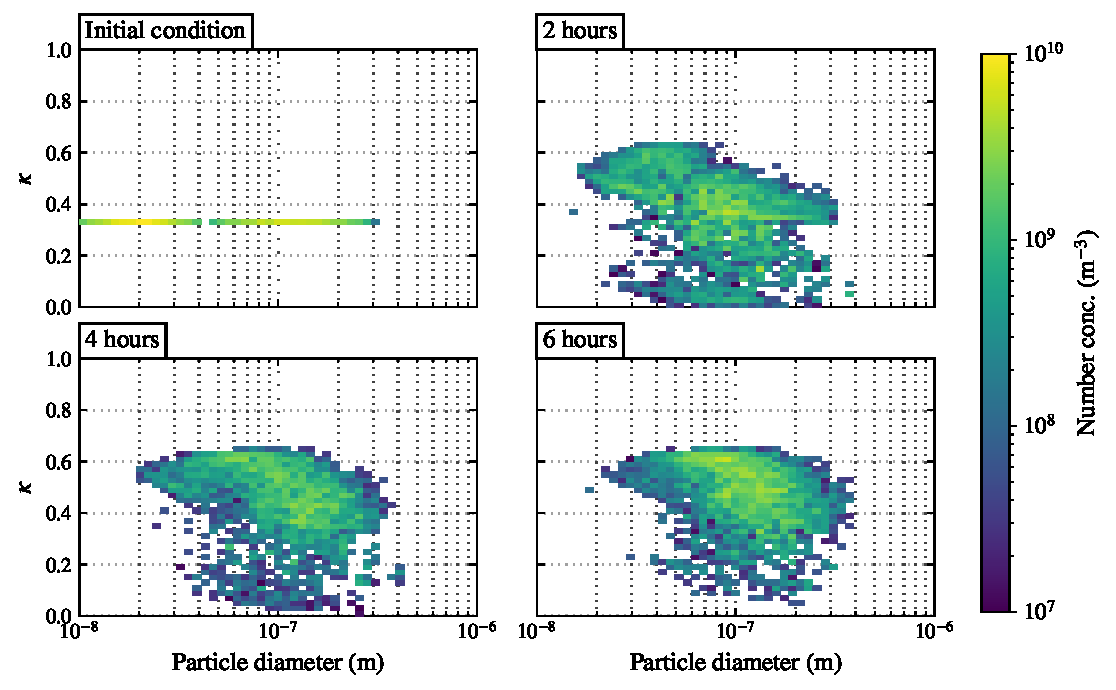
\includegraphics[width=\textwidth]{figures/chapter5/2d-kappa-dist-4-panel-point-source-1x1-z40.pdf}
    \caption{2-dimensional number distributions $n(D_p, \kappa)$ at regular two-hour intervals for scenario~3.}
    \label{fig:2d-kappa-dist-s3}
\end{figure}

Figure \ref{fig:2d-kappa-dist-s3} shows two-dimensional size distributions at regular two hour intervals for the highest $SH$ scenario, scenario~3. We find that following the initial condition, the evolution of the $\kappa$-resolved size distribution differs markedly from the uniform base case in numerous ways. First, the abundance of low-$\kappa$ primary aerosol due to emissions is greatly reduced for $t=2$ h to $t=6$ h. The increased rate of coagulation for high $SH$ scenarios shown in Section \ref{ideal-coag-results} indicates that this process is likely enhanced for emissions scenario~3 and removes aerosol particles in the high-concentration emissions plume. Additionally, we find a greater abundance of high-$\kappa$ particles in the size range 20 nm to 0.4 \si{\mu m} with $\kappa$ in excess of 0.6 for some particles near $D_p=0.1$ \si{\mu m}. By comparison, far fewer particles in the uniform base case possess $\kappa\approx0.6$ and are limited to the size range 20--30 nm. 

\subsection{Aerosol mixing state}

\begin{figure}[!t]
  \centering
    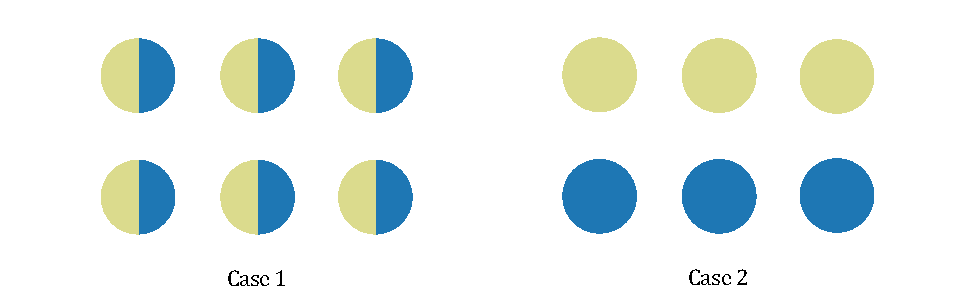
\includegraphics[width=\textwidth]{figures/chapter5/mixing-state-ideal-cases.pdf}
    \caption{Two idealized cases for aerosol populations composed of ammonium sulfate (blue) and organic carbon (beige). Case 1 is fully internally mixed while case 2 is fully externally mixed, yet each case contains the same bulk concentration of each species.}
    \label{fig:mixing-state-scenarios}
\end{figure}

So far in this section we have shown results for the bulk and size-resolved composition of the aerosol. That is, we have shown which aerosol species are contained in the population, their mean abundances, and how they vary with particle size. However, these results do not indicate how each aerosol species is distributed amongst the particles in the population. Consider two cases, each with a grouping of six monodisperse aerosol particles. In the first case, all aerosol particles are an equal mixture of 50\% ammonium sulfate and 50\% OC. In the second case, half of the particles are 100\% ammonium sulfate and the remaining half are 100\% OC. When averaged to find the bulk composition of the population, each case leads to the same conclusion--the population is composed of 50\% ammonium sulfate and 50\% OC. However, this bulk state oversimplifies the compositional diversity of the particle population and aerosol particle properties vary considerably across each case. Note that the hygroscopicity $\kappa$ of each particle differs across both cases. If all particles are internally mixed as in the first case (i.e., each particle is a mixture of ammonium sulfate and OC), the hygroscopicity of all particles will be $\kappa=0.33$. For the second case, the particles are externally mixed (i.e., each particle is purely composed of a single aerosol species), resulting in the ammonium sulfate particles being highly hygroscopic, $\kappa=0.65$, while the pure OC particles are nearly nonhygroscopic, $\kappa=0.001$. As a consequence, there will exist a supersaturation at which all of the particles in case 1 active as CCN, while only half of the particles in the second case will active. This illustrates the importance of the aerosol mixing state, which describes how externally or internally mixed aerosol species are in the particle population. 

The mixing state $\chi$ is quantified using the metric definition of \textcite{riemer_quantifying_2013} and is defined as 
\begin{equation}
\chi = \frac{D_{\alpha}-1}{D_{\gamma}-1},
\end{equation}
where $D_{\alpha}$ is the average particle species diversity and $D_{\gamma}$ is the bulk population species diversity. $D_{\alpha}$ is related to the average Shannon entropy for each particle as 
 \begin{equation}
D_{\alpha} = \exp\left(\sum_{i=1}^N p_i H_i\right),
\end{equation}
where $p_i$ is the mass fraction of particle $i$ in the population and $H_i$, the Shannon entropy of the species distribution in particle $i$, is 
\begin{equation}
H_i = \sum_{a=1}^A -p_i^a\ln(p_i^a),
\end{equation}
where $p_i^a$ is the mass fraction of species $a$ in particle $i$.

$D_{\gamma}$ is related to the Shannon entropy for the distribution of an aerosol species in the population as 
 \begin{equation}
D_{\gamma} = \exp\left(\sum_{a=1}^A p^a \ln(p^a)\right),
\end{equation}
where $p^a$ is the mass fraction of species $a$ in the population.

\begin{figure}[!t]
  \centering
    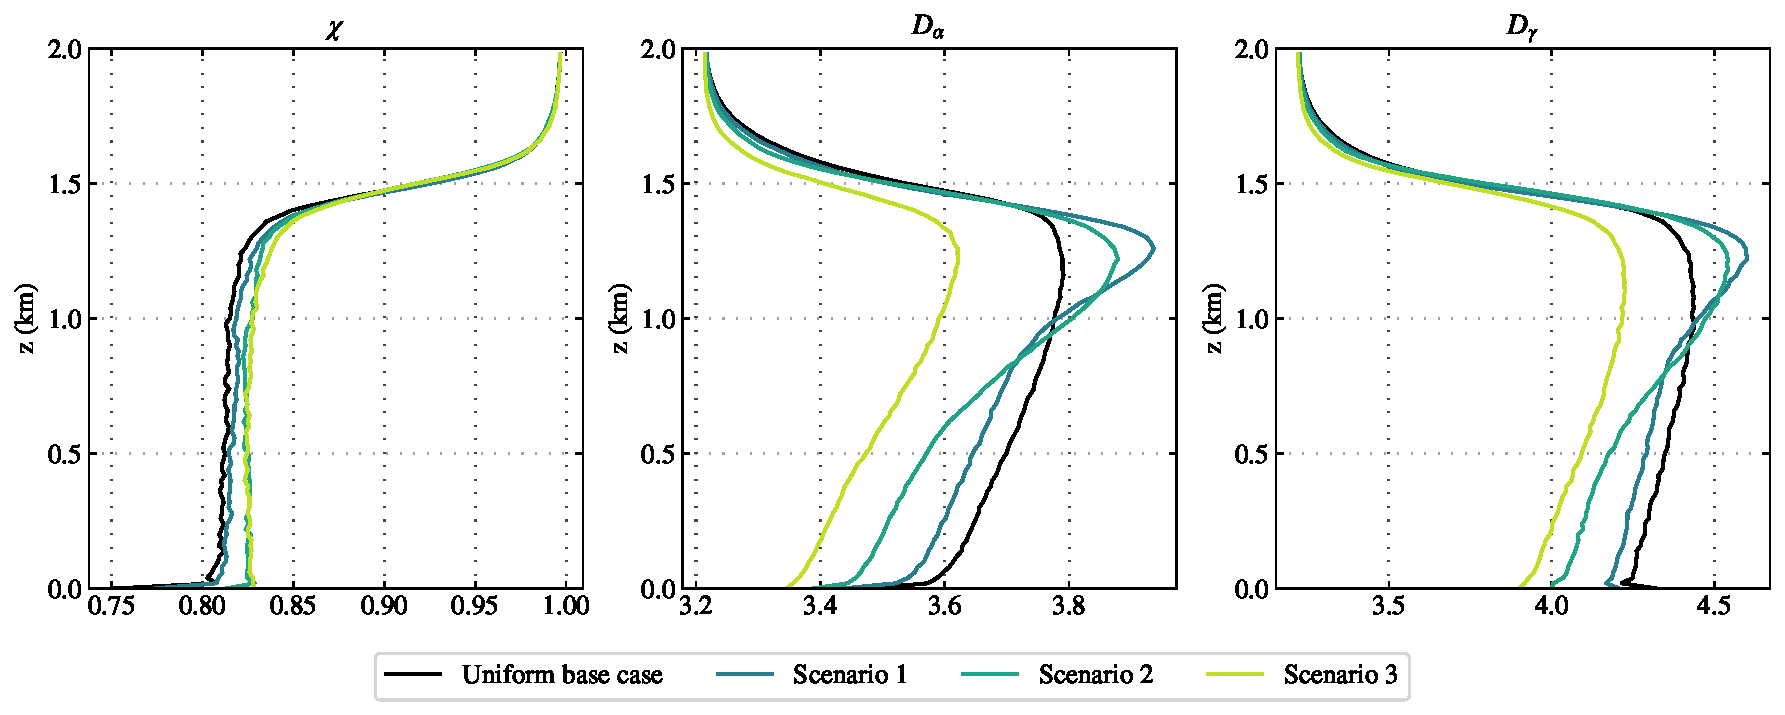
\includegraphics[width=\textwidth]{figures/chapter5/aerosol-mixingstate-vertical-profiles-time36.pdf}
    \caption{Vertical profiles for mixing state $\chi$ and diversity measures $D_{\alpha}$ and $D_{\gamma}$ for each emissions scenario at $t=6$ h.}
    \label{fig:mixing-state-vert-profiles}
\end{figure}

Figure \ref{fig:mixing-state-vert-profiles} shows vertical profiles for $\chi$ and its associated diversity measures $D_{\alpha}$ and $D_{\gamma}$ for each emissions scenario at $t=6$ h. We find that $\chi$ is approximately the same across each emission scenario in both the planetary boundary layer and in the free troposphere. Furthermore, $\chi$ is nearly uniform within the planetary boundary layer, with values near $\chi\approx0.81$ in the uniform base case and $\chi\approx0.83$ in the highest $SH$ scenario, scenario~3. Above the planetary boundary layer, $\chi$ matches closely across all scenarios and reaches $\chi\approx1$ by the top of the domain. These results point to a near-fully internally mixed aerosol population in the planetary boundary layer and completely internally mixed aerosol above the planetary boundary layer. 

We find that diversity measures $D_{\alpha}$ and $D_{\gamma}$ increase with height in the planetary boundary layer and subsequently decrease in the free troposphere. In the middle to lower planetary boundary layer, both $D_{\alpha}$ and $D_{\gamma}$ decrease for high $SH$ scenarios relative to the uniform base case. We find that $D_{\alpha}$ and $D_{\gamma}$ both peak near the top of the planetary boundary layer and reach a maximum for emissions scenario~1 at 3.95 and 4.6, respectively. 

\begin{figure}[!t]
  \centering
    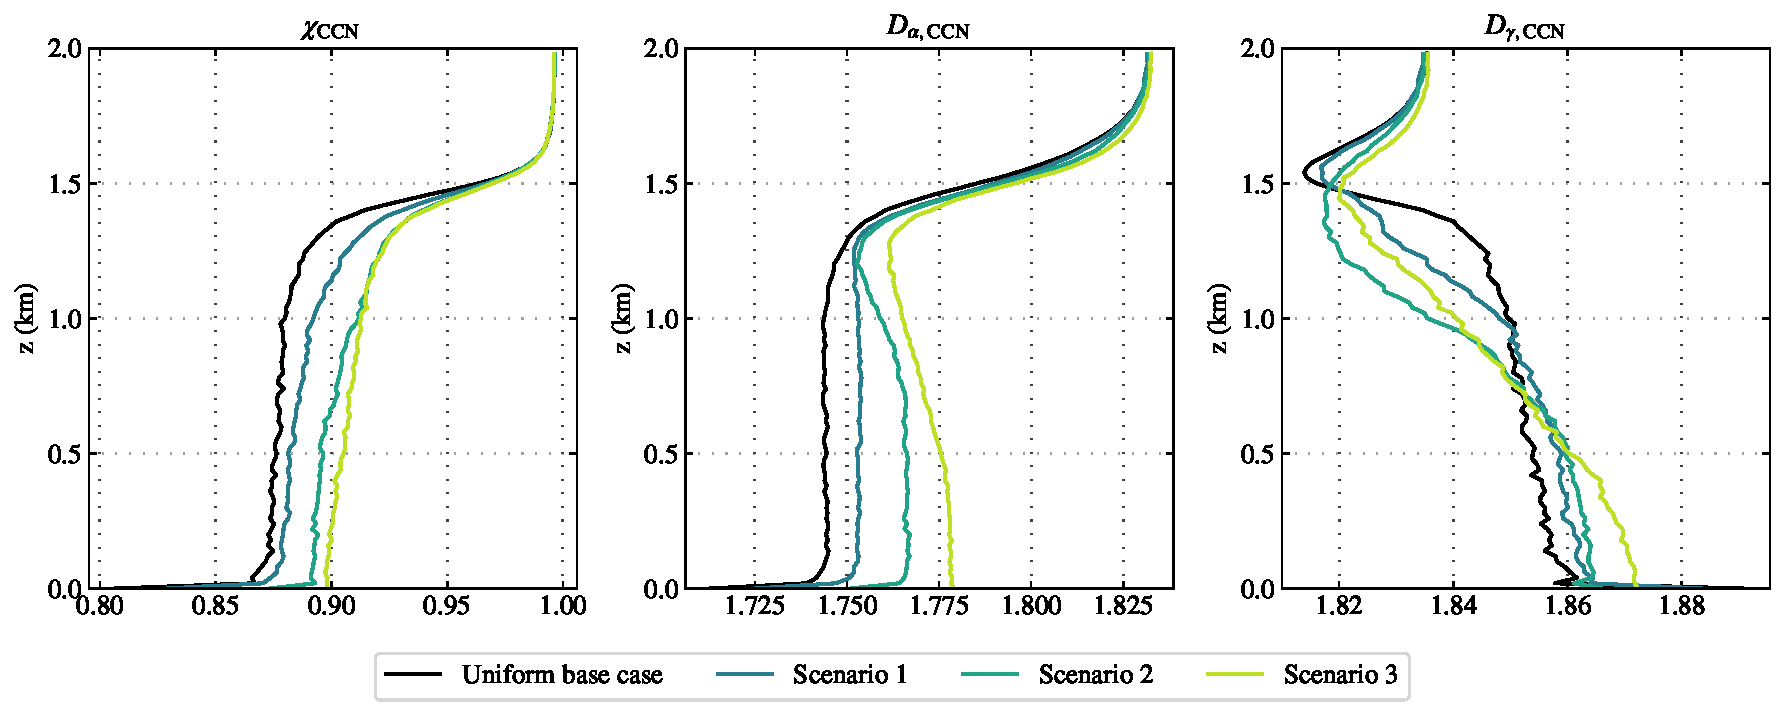
\includegraphics[width=\textwidth]{figures/chapter5/aerosol-ccn-mixingstate-vertical-profiles-time36.pdf}
    \caption{Vertical profiles for CCN mixing state $\chi_{\text{CCN}}$ and diversity measures $D_{\alpha,\text{CCN}}$ and $D_{\gamma,\text{CCN}}$ for each emissions scenario at $t=6$ h.}
    \label{fig:ccn-mixing-state-vert-profiles}
\end{figure}

Figure \ref{fig:ccn-mixing-state-vert-profiles} shows vertical profiles for $\chi$ and diversity measures $D_{\alpha}$ and $D_{\gamma}$ for particles which activate as CCN. $\chi_{\text{CCN}}$ and the corresponding diversity measures are calculated by grouping hydrophobic species (BC and OC) and hydrophilic species (all remaining species). Thus $D_{\alpha,\text{CCN}}$ and $D_{\gamma,\text{CCN}}$ range between 1 and 2. For each emissions scenario, $\chi_{\text{CCN}}$ gradually increases in the planetary boundary layer. $\chi_{\text{CCN}}$ is slightly greater than $\chi$ for each scenario, indicating that CCN are very well mixed in the planetary boundary layer. Furthermore, $\chi_{\text{CCN}}$ increases slightly with greater emissions $SH$ (e.g., at $z=500$ m, $\chi_{\text{CCN}} = 0.87$ for the uniform base case and $\chi_{\text{CCN}} = 0.90$ for scenario~3). As $SH$ increases, $D_{\alpha,\text{CCN}}$ also slightly increases in the planetary boundary layer (e.g., at $z=500$ m, $D_{\alpha,\text{CCN}} = 1.74$ for the uniform base case and $D_{\alpha,\text{CCN}} = 1.77$ for scenario~3). Above the planetary boundary layer, $D_{\alpha,\text{CCN}}$ tends to converge across emissions scenarios, increasing to $\approx1.83$ at $z=2$ km. We find that $D_{\gamma,\text{CCN}}$ gradually decreases moving vertically in the planetary boundary layer for each emissions scenario. As $SH$ increases across emissions scenarios, $D_{\gamma,\text{CCN}}$ takes on higher values in the lower to middle boundary layer, while in the middle to upper boundary layer this trend is reversed, with higher $SH$ indicating lower values of $D_{\gamma,\text{CCN}}$. 

\subsection{Impacts of emissions $SH$ on CCN activity}

We have shown that emissions spatial heterogeneity alters the aerosol composition, producing more nitrate-rich particles and that this results in an increase in aerosol hygroscopicity $\kappa$. The critical supersaturation at which a particle activates as a cloud condensation nucleus is a function of $\kappa$ and particle diameter. Thus, changes to the aerosol properties such as composition and hygroscopicity will propagate to changes in CCN activity. 

Here, we group particles by critical saturation into CCN that activate at the following supersaturation levels:  $S=0.1, 0.3, 0.6, 1.0\%$. CCN concentrations at each supersaturation level are determined in the following manner. First, the critical supersaturation $S_c$ is determined for each particle by using a root finding algorithm to solve for the critical point of the supersaturation curve $S(D_p, \kappa)$ of $\kappa$-Köhler theory \parencite{petters_single_2007}. Particles are then grouped by supersaturation ($0.1, 0.3, 0.6, 1.0\%$) required for activation in a cumulative manner (i.e., particles activating at $S=0.3\%$ are included in bins for $S=0.5\%$ and higher supersaturations as they will activate at any supersaturation higher than $S=0.3\%$). Subsequently, the concentration of CCN at each supersaturation level is determined for each grid cell. 

Figure \ref{fig:vertprof-ccn} shows vertical profiles for each emissions scenario of CCN that activate at supersaturations $S=0.1, 0.3, 0.6, 1.0\%$. Each vertical profile is taken at time $t=6$ h and displays the level-averaged mixing ratio in ppbv of particles that would act as CCN at each supersaturation level (note, environmental conditions do not exceed 100\% RH at any point or time in each simulation).  

For $S=0.1\%$, we find that CCN concentrations decrease with increasing $SH$ in the lower boundary layer. In the middle to upper boundary layer, the opposite trend is observed, with CCN concentrations increasing as emissions $SH$ increases. This increase is most pronounced at the top of the planetary boundary layer ($z\approx 1.25$ km), where CCN concentrations reach nearly 1.2 ppbv for scenario~3 compared to 1.0 ppbv in the uniform base case. 

Increases in CCN concentrations due to increasing emissions $SH$ are observed everywhere in the planetary boundary layer for $S=0.3\%$, with concentrations again peaking near the top of the boundary layer. For the highest $SH$ scenario, we find CCN concentrations in the upper planetary boundary layer exceed 3.5 ppbv, while in the uniform base case, CCN concentrations are a vertically uniform 2.8 ppbv. 

\begin{figure}[!t]
  \centering
    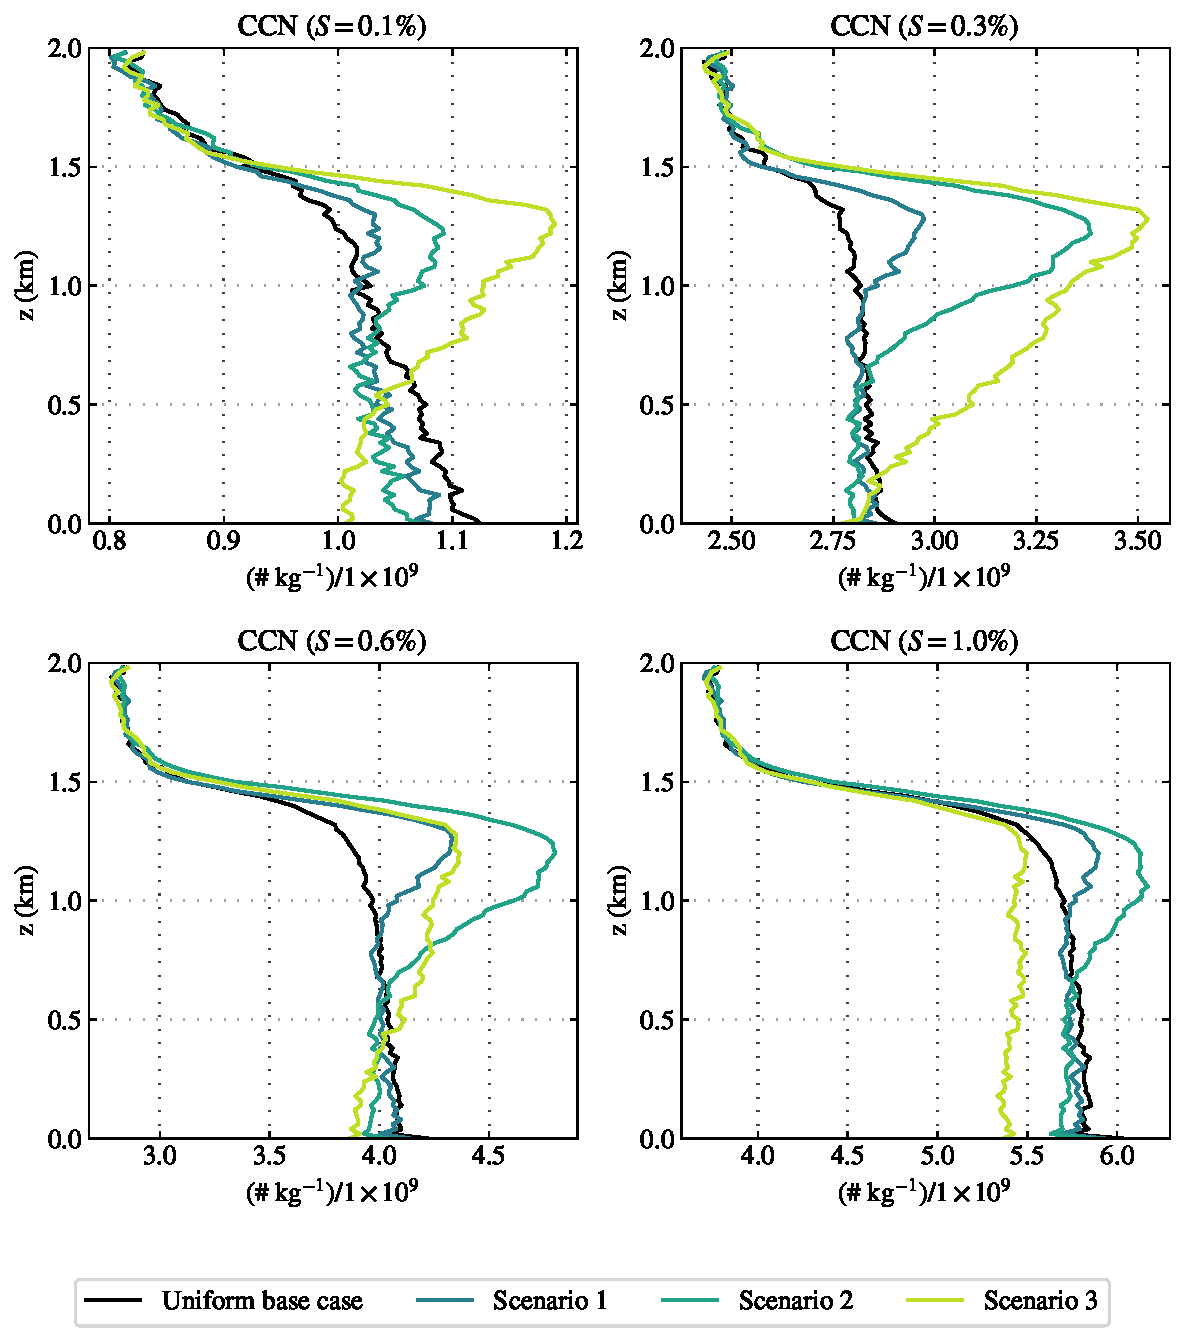
\includegraphics[width=.9\textwidth]{figures/chapter5/aerosol-ccn-vertical-profiles-time36.pdf}
    \caption{Vertical profiles ($t=6$ h) for each emission scenario of CCN activating at supersaturations $S=0.1, 0.3, 0.6, 1.0$\%}
    \label{fig:vertprof-ccn}
\end{figure}

For $S=0.6\%$, we find that CCN concentrations in the lowest 500 m of the planetary boundary layer for Scenarios 1--3 are slightly lower than in the uniform base case. In the middle to upper planetary boundary layer, we find that the increases in $SH$ correspond to non-monotonic changes in CCN concentrations (i.e., CCN concentrations do not appear to increase with progressively higher $SH$ scenarios as found in the upper planetary boundary layer for $S=0.1\%$ and $S=0.3\%$). Instead, CCN concentrations in the upper planetary boundary layer for $S=0.6\%$ are highest for the mid-$SH$ scenario (scenario~2), followed by scenario~3, scenario~1, and the uniform base case. 

For $S=1.0\%$ we also find a complex set of responses to CCN concentrations across emissions $SH$ scenarios. For low to mid-$SH$ scenarios 1 and 2, we find that CCN concentrations in the lowest $600$ m of the planetary boundary layer closely align with the uniform base case. In the middle to upper boundary layer, scenarios 1 and 2 exhibit an increase in CCN concentrations relative to the uniform base case. We find that CCN concentrations for $S=1.0\%$ in the highest $SH$ scenario, scenario~3, are approximately uniform throughout the extent of the planetary boundary layer at 4.4 ppbv, slightly less than the 4.6 ppbv observed for the uniform base case. 

\begin{figure}[!t]
  \centering
    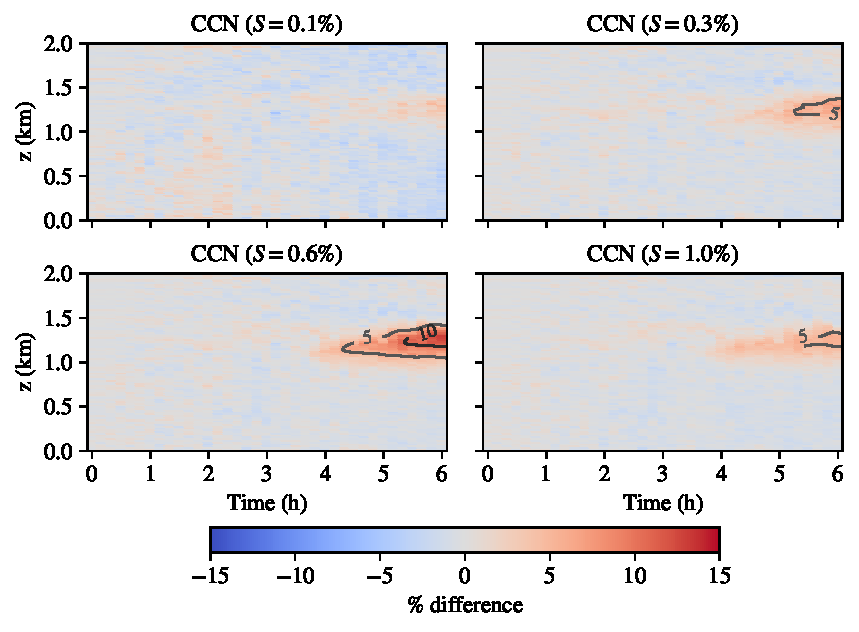
\includegraphics[width=\textwidth]{figures/chapter5/height-time-ccn-pdiff-fx1fy0.pdf}
    \caption{Time-height plots for the percent difference between CCN concentrations in the uniform base case and scenario~1 for each supersaturation level. Red indicates an increase in CCN relative to the base case while blue indicates a decrease. Isopleths indicate lines of constant percent difference in increments of 5\%.}
    \label{fig:ht-ccn-pdiff-s1}
\end{figure}

Figure \ref{fig:ht-ccn-pdiff-s1} shows time-height plots for the percent difference of CCN concentrations in emissions scenario~1 relative to the uniform base case. Plots are shown for each supersaturation level ($S=0.1, 0.3, 0.6, 1.0\%$). Red indicates increases in CCN concentrations relative to the base case while blue indicates a decrease. To aid interpretability, isopleths indicating percent difference in steps of $5\%$ are shown on each figure. If no isopleths are present, this indicates that percent difference did not exceed $5\%$ anywhere or at any time between the emissions scenario CCN concentrations and the uniform base case. Percent difference is calculated as 
\begin{equation}
    \% \text{ difference} = 100\times\left(\frac{\overline{[\text{CCN}]}(t, z, S)_{\text{Scenario}} - \overline{[\text{CCN}]}(t, z, S)_{\text{Base case}}}{\overline{[\text{CCN}]}(t, z, S)_{\text{Base case}}}\right),
\end{equation}
where $\overline{[\text{CCN}]}(t, z,S)_{\text{Scenario}}$ is the horizontally averaged concentration of CCN at time $t$ and vertical level $z$ that activate at supersaturation $S$ for the given emissions scenario and $\overline{[\text{CCN}]}(t, z, S)_{\text{Base case}}$ is the horizontally averaged concentration of CCN at time $t$ and vertical level $z$ that activate at supersaturation $S$ for the uniform base case.

Stepping through each supersaturation level, we find that at $S=0.1\%$, percent difference does not exceed 5\% at any point during the simulation. Slight spatial and temporal fluctuations are found in CCN concentrations, however, these do not appear to significantly depart from percent difference between scenario~1 and the uniform base case in the first hour of the simulation during which the configuration and spinup of each simulation is identical, indicating that internal variability due to stochastic noise is likely on the order of 1--2\%.

For $S=0.3\%$, we find a slight increase in CCN concentrations beginning at $t=5$ h from $z\approx1.1$ km to $z\approx1.4$ km on the order of 5\%. Similarly for $S=0.6\%$ and $S=1.0\%$, we find that CCN concentrations increase in the upper planetary boundary layer. At $S=0.6\%$ CCN concentrations increase up to 10\% by $t=5$ h. At $S=1.0\%$, we find similar behavior in the percent difference for $S=0.3\%$, with an increase in CCN concentrations the upper planetary boundary layer of up to 5\%.

\begin{figure}[!t]
  \centering
    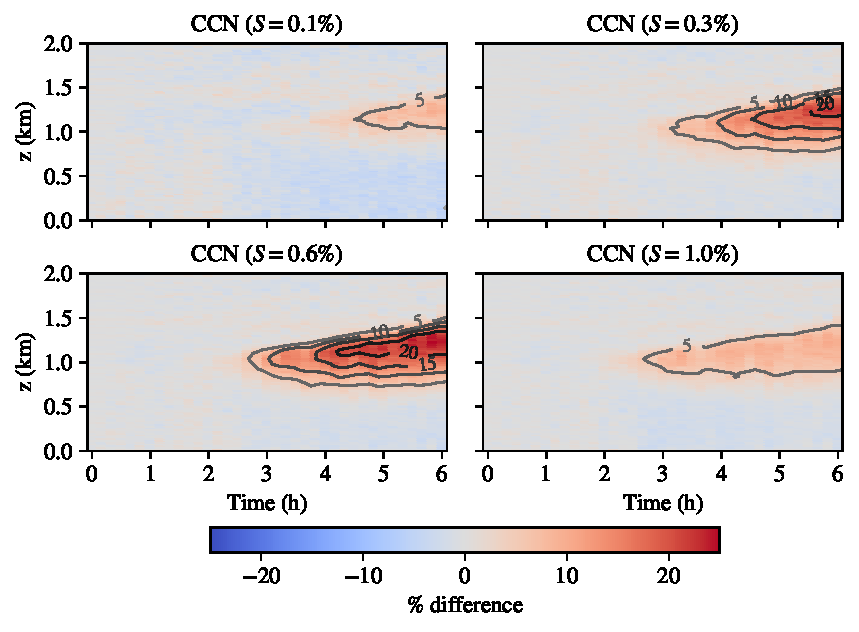
\includegraphics[width=\textwidth]{figures/chapter5/height-time-ccn-pdiff-road-10x.pdf}
    \caption{Time-height plots for the percent difference between CCN concentrations in the uniform base case and scenario~2 for each supersaturation level. Red indicates an increase in CCN relative to the base case while blue indicates a decrease. Isopleths indicate lines of constant percent difference in increments of 5\%.}
    \label{fig:ht-ccn-pdiff-s2}
\end{figure}

Figure \ref{fig:ht-ccn-pdiff-s2} shows time-height plots for percent difference in CCN concentrations at each supersaturation level between scenario~2 and the uniform base case. We find that for each supersaturation level, CCN concentrations increase in the upper planetary boundary layer by at least 5\%. Additionally, the onset of increased CCN concentrations relative to the uniform base case is earlier than found for scenario~1 for each supersaturation level. 

For $S=0.1\%$, we find that CCN concentrations in the upper planetary boundary layer increase up to 5\% beginning at $t=4.5$ h. For $S=0.3\%$ and $S=0.6\%$, we find increases of up to 20\% with elevated concentrations relative to the uniform base case beginning at $t\approx3$ h and gradually increasing in the upper planetary boundary layer through the remainder of each simulation. For $S=1.0\%$, CCN concentrations increase in a similar manner to those found for $S=0.1\%$ with concentrations increasing up to 5\% in the upper planetary boundary layer. However, CCN concentrations increase earlier than in the lower supersaturation case, with elevated concentrations by 5\% in the upper planetary boundary layer appearing around $t=2.5$ h.

\begin{figure}[!t]
  \centering
    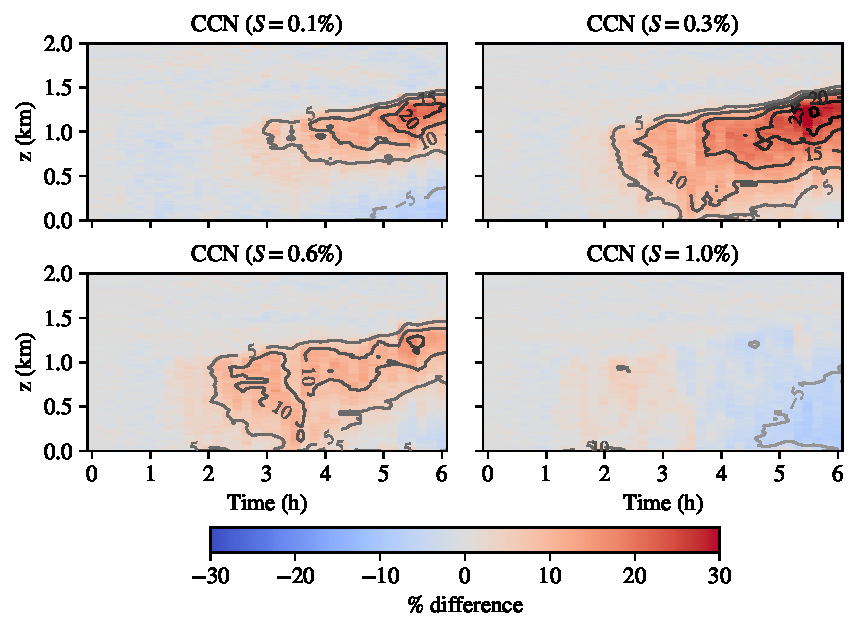
\includegraphics[width=\textwidth]{figures/chapter5/height-time-ccn-pdiff-point-source-1x1.pdf}
    \caption{Time-height plots for the percent difference between CCN concentrations in the uniform base case and scenario~3 for each supersaturation level. Red indicates an increase in CCN relative to the base case while blue indicates a decrease. Isopleths indicate lines of constant percent difference in increments of 5\%.}
    \label{fig:ht-ccn-pdiff-s3}
\end{figure}

Figure \ref{fig:ht-ccn-pdiff-s3} displays time-height plots for percent difference in CCN concentrations at each supersaturation level between scenario~3 and the uniform base case. 
Compared with scenarios 1 and 2, the trend of increasing CCN concentrations is much more vertically and temporally vaired, particularly for $S=0.3\%$ and $S=0.6\%$ where an increase in CCN concentrations begins in the upper planetary boundary layer at $t=2$ h, extends downward throughout the vertical extent of the planetary boundary layer by $t=3$ h, and moves back upwards towards the mid to upper planetary boundary layer beginning at $t=4$ h. 

For $S=0.1\%$, CCN concentrations increase by up to 20\% in the upper boundary layer by $t=5.5$ h. Beginning around $t=5$ h, CCN concentrations decrease by up to 5\% in the lowest 300 m of the domain. At $S=0.3\%$, CCN concentrations increase by up to 25\% in the upper planetary boundary layer beginning at $t=5$ h. This is the highest magnitude CCN concentration percent difference observed for any supersaturation and across any emissions scenario. For $S=0.6\%$, CCN concentrations increase by 10--15\%, indicating a notable drop in the magnitude of elevated CCN concentrations when compared to scenario~2 results for $S=0.6\%$ shown in Figure \ref{fig:ht-ccn-pdiff-s2}. At $S=1.0\%$, we find a slight reduction in CCN concentrations by up to 5\% that starts near the surface at $t\approx4.5$ h and extends throughout the lower to middle planetary boundary layer by $t=6$ h. 

\subsection{Influence of ammonia on aerosol composition and CCN activity}

We have shown that the composition of the aerosol population varies considerably with emissions spatial heterogeneity. Specifically, nitrate and ammonium are found to substantially increase as emissions $SH$ increases. Changes in the relative abundance of these species alters the hygroscopic properties of the aerosol resulting in an increased concentration of CCN at low supersaturations. 

Sulfate and nitrate are both anions with charge $-2$ and $-1$, respectively, while ammonium is an cation with charge +1. In turn, ammonium plays an important role in neutralizing both sulfate and nitrate. Due to the extremely low volatility of H$_2$SO$_4$, it rapidly partitions into the aerosol phase where it dissociates into SO$_4^{-2}$. In turn, available ammonia will first partition into the aerosol phase and neutralize sulfate by forming ammonium sulfate. Any remaining ammonia in excess of what is required to neutralized the sulfate, referred to as free ammonia, will enter the aerosol and bind to nitrate, thus forming ammonium nitrate. Crucially, the abundance of free ammonia determines the concentration of nitrate in the aerosol phase; if no free ammonia is available then no nitrate will enter the aerosol, whereas the presence of free ammonia allows a one-to-one molar ratio of nitrate to ammonium in the form of ammonium nitrate.  

Here, we run two additional modified simulations for the uniform base case and scenario~3 in which the concentration of total ammonium ($\text{NH}_{3\text{, gas}} + \text{NH}_{4\text{, aerosol}}$) is set to zero. Emissions of NH$_3$ are also set to zero to ensure that total ammonium remains zero throughout each simulation. These additional simulations help to isolate the impact of emissions spatial heterogeneity on aerosol composition and CCN activity in the absence of ammonium.  

\begin{figure}[!t]
  \centering
    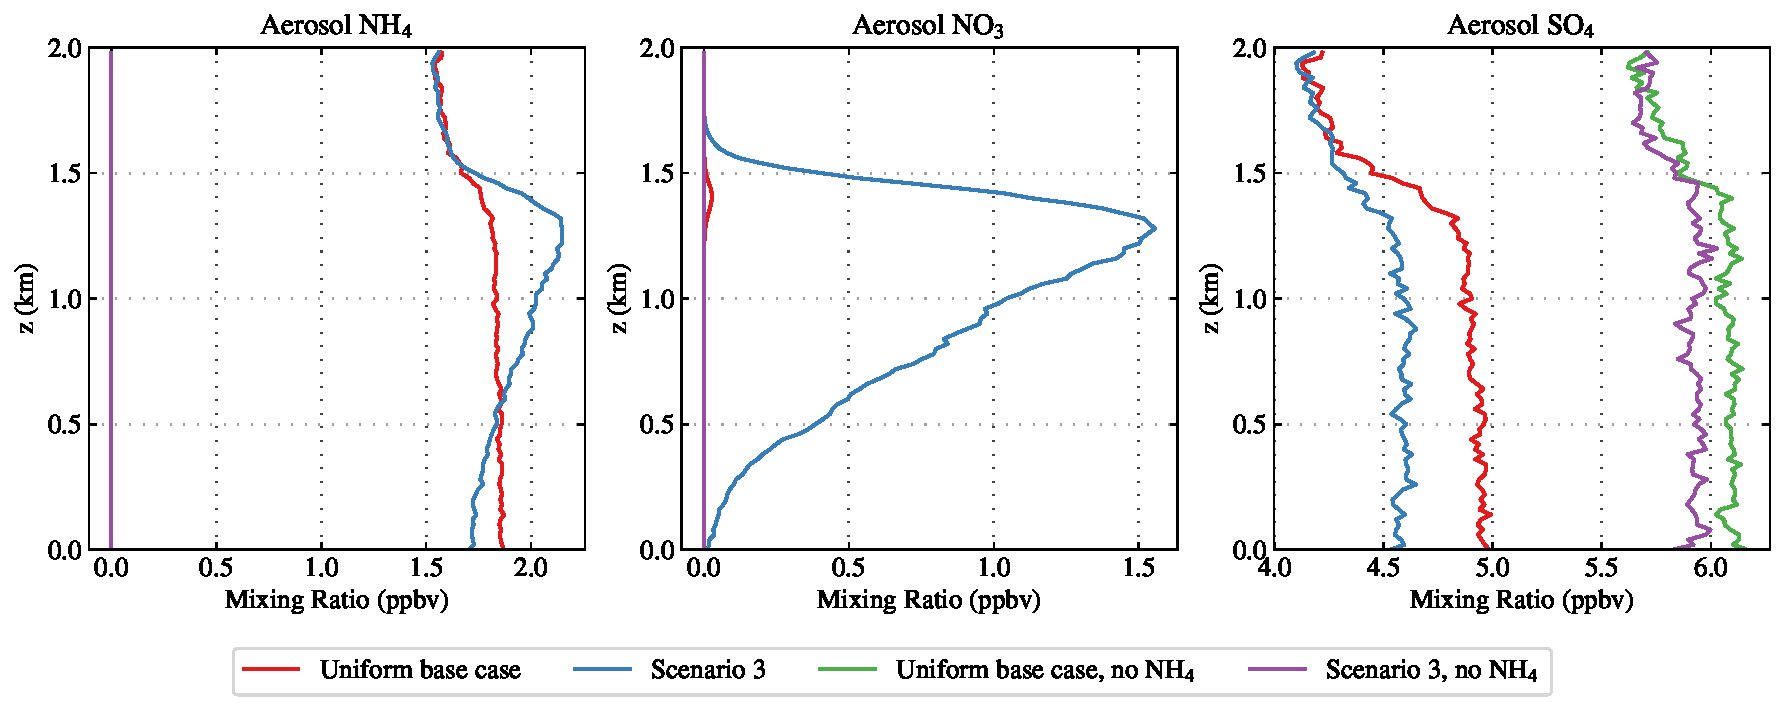
\includegraphics[width=\textwidth]{figures/chapter5/aerosol-SNA-vertical-profiles-no-nh4-cases-time36.pdf}
    \caption{Vertical profiles ($t=6$ h) for ammonium, nitrate, and sulfate comparing uniform base case and scenario~3 both with and without ammonium.}
    \label{fig:vert-profiles-no-nh4}
\end{figure}

Figure \ref{fig:vert-profiles-no-nh4} shows vertical profiles at $t=6$ h for aerosol ammonium, nitrate, and sulfate concentrations in ppbv for four simulation runs: the uniform base case and scenario~3 as shown in previous sections and the same scenarios but without any ammonium present. Simulations with ammonium show that the uniform base case has slightly more ammonium in the lowest 500 m of the planetary boundary layer, while scenario~3 has higher concentrations in excess of 2 ppbv in the middle to upper planetary boundary layer. As a consistency check, the same scenarios without ammonium (uniform base case in green, scenario~3 in purple) indicate zero ammonium throughout the entire domain. We find that simulations without ammonium contain no nitrate, which is consistent with previous discussion of the availability of free ammonia in order to allow nitrate to enter the aerosol phase. Without ammonium present, sulfate concentrations increase for both the uniform base case (4.9 ppbv to 6.1 ppbv) and scenario~3 (4.6 ppbv to 5.9 ppbv).

\begin{figure}[!t]
  \centering
    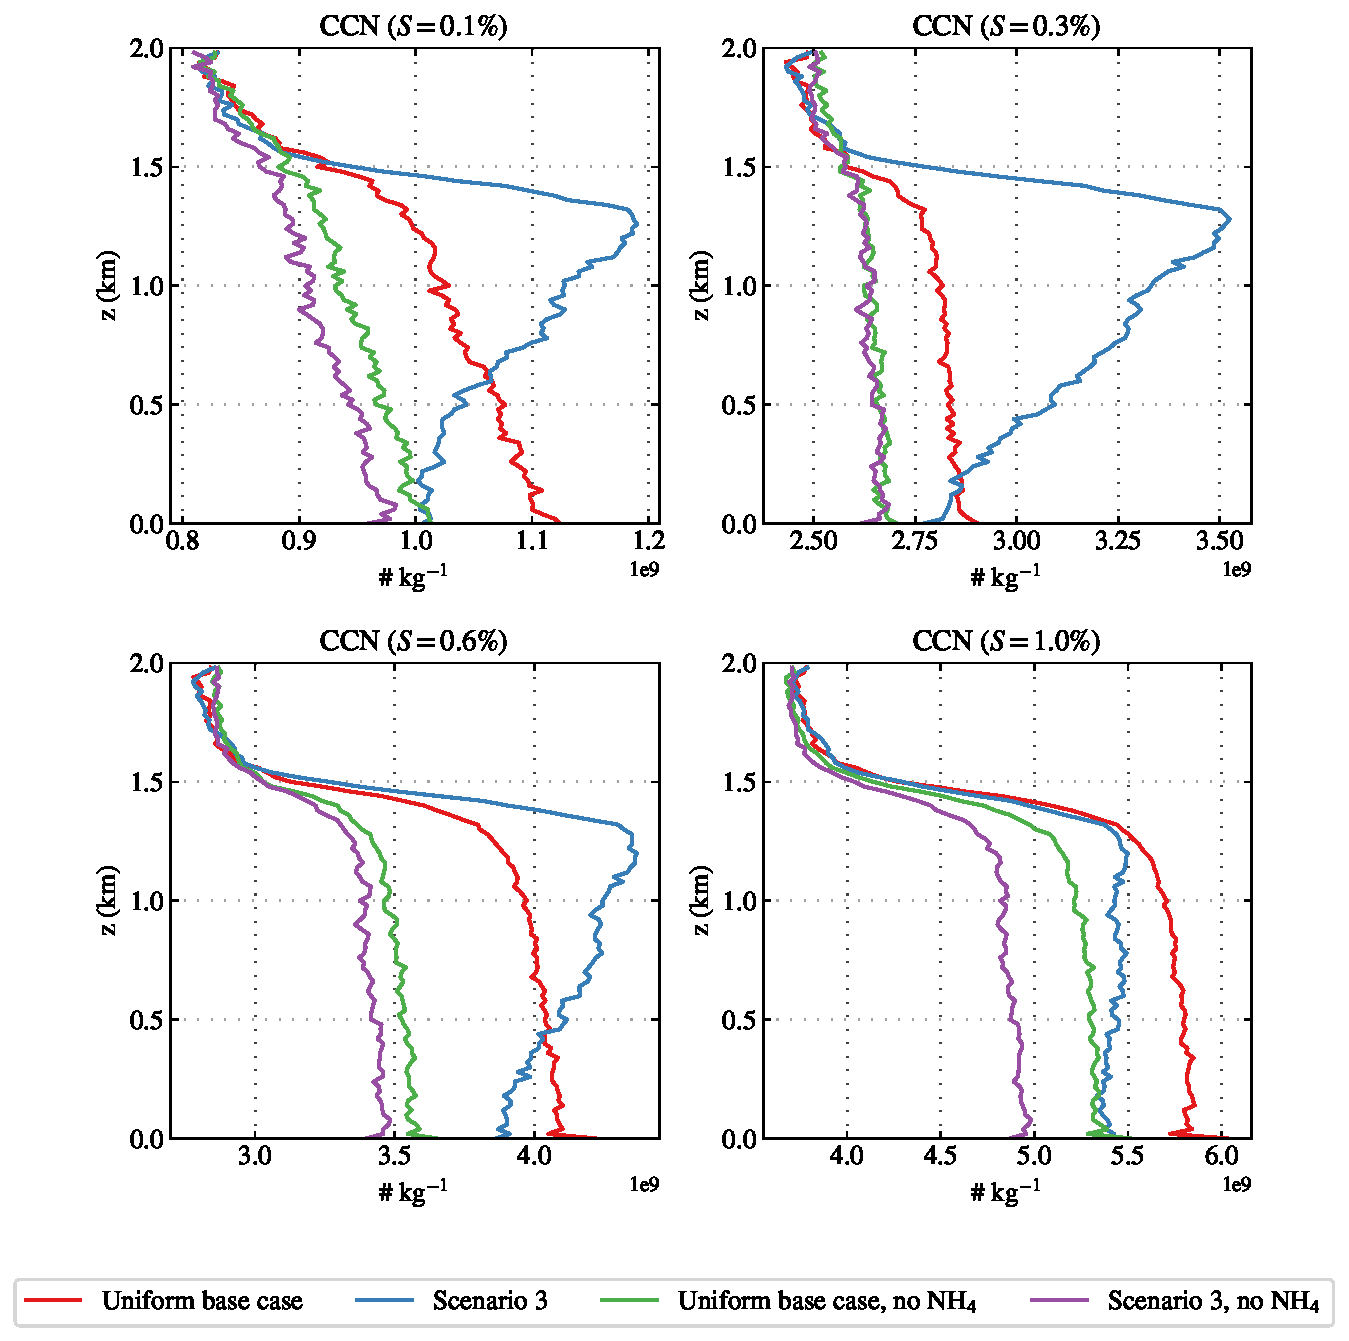
\includegraphics[width=\textwidth]{figures/chapter5/aerosol-ccn-vertical-profiles-no-nh4-cases-time36.pdf}
    \caption{Vertical profiles ($t = 6$ h) for CCN concentrations at supersaturations S = 0.1, 0.3, 0.6, 1.0\% for the uniform base case and scenario~3 with and without ammonium.}
    \label{fig:vert-profiles-ccn-no-nh4}
\end{figure}

Figure \ref{fig:vert-profiles-ccn-no-nh4} shows vertical profiles of CCN number concentrations in ppbv at $t=6$ h for each supersaturation level (S = 0.1, 0.3, 0.6, 1.0\%) for both the uniform base case and emissions scenario~3 with and without ammonium. We find that in the absence of ammonium, concentrations of CCN at each supersaturation level agree closely across the uniform base case and scenario~3. For $S=0.1\%$, we find that CCN concentrations in scenario~3 (no ammonium) are a constant factor of $0.02\cdot10^{18}$ ppbv less than in the uniform base case (no ammonium). At $S=0.3\%$, CCN concentrations across both scenarios are virtually identical to within random variability. For $S=0.6\%$, the no-ammonium scenario~3 has a relatively constant factor of $0.1\cdot10^{18}$ ppbv less CCN than the no-ammonium uniform base case. We find a similar relationship for $S=1.0\%$ with a constant factor of $0.5\cdot10^{18}$ ppbv fewer CCN in the ammonium-free scenario~3 case. 

%\hl{I think it would be helpful here to include profiles of total number concentration > 50 nm (could also do this elsewhere). My thinking is that coagulation is probably reducing the total number of particles in the high heterogeneity case and this leads to the lower CCN conc. I think this is somewhat counteracted by the increased hygroscopicity of particles in the set of scenarios with ammonium/nitrate present in the aerosol.}

\section{Implications}

%Non-linear coupling between emissions $SH$ and CCN activity, mediated by the presence of nitrate and contingent on the availability of free ammonia to allow partitioning of nitrate into the aerosol phase.

Idealized coagulation simulations indicate that higher emissions spatial heterogeneity leads to a higher rate of coagulation due to increased number concentration. Correspondingly, number distributions for full mulitphase chemistry simulations indicate a reduction in smaller emission-mode particles and a shift to larger particles likely in part due to enhanced coagulation.

Sulfate concentrations are lower for high emissions heterogeneity scenarios. This results from the partitioning of less H$_2$SO$_4$ into the aerosol phase. Because H$_2$SO$_4$ possesses a very low volatility vapor pressure, nearly all available H$_2$SO$_4$ will enter the aerosol to form sulfate. This indicates that the availability of sulfate is controlled by the gas phase oxidation of SO$_2$ to form H$_2$SO$_4$ via OH, and that less OH reacts with SO$_2$ under high emissions heterogeneity scenarios. 

There are numerous contributing factors which alter the availability of OH, first of which is the emissions heterogeneity of the plume. In high heterogeneity scenarios where concentrations in the emissions plume are very high, OH near the vicinity of the plume will rapidly react with the plume constituents including SO$_2$, NO$_x$, and VOCs. This quickly strips the availability of OH in the core of the plume. Reactions including photolytic processes outside the plume that produce OH are not able to replenish the concentration of OH near the plume due to an inability to mix and entrain OH into the plume fast enough. As a result, OH is chemically segregated from its reactants in the plume including SO$_2$. 

In addition to impacts of emissions plume spatial heterogeneity and chemical segregation, the availability of OH in high emissions heterogeneity scenarios may also be reduced due to lower concentrations of ozone as found in chapter 4. The photolysis of ozone into singlet oxygen and subsequent reaction with H$_2$O is an important formation mechanism for OH. In addition to the mechanism responsible for the reduction in the abundance of ozone discussed in chapter 4, it is likely that aerosols alter the rate of photolysis reactions by increased scattering and absorption of radiation. As many formation mechanisms for OH require photolysis, high concentrations of aerosol particles likely reduces the effective rate at which photolytic reactions occur, especially near the emissions plume. 

We find that both ammonium and nitrate concentrations increase with emissions spatial heterogeneity, particularly in the upper boundary layer.  Note that most ammonium and nitrate are present in the aerosol phase as ammonium nitrate, which forms via the gas-solid equilibrium reaction between nitric acid and ammonia in the gas phase to form solid ammonium nitrate. Note that nitric acid forms by reacting ozone with NO$_2$. The higher concentrations of NO$_2$ observed for high emissions spatial heterogeneity scenarios in chapter 4 indicates an increase in nitric acid (if there is enough OH). The nitric acid-ammonium equilibrium reaction is highly sensitive to temperature with more ammonium nitrate formation at lower temperatures. This helps explain why ammonium and nitrate levels are the highest in the upper boundary layer. Furthermore, the decrease in sulfate under high emissions heterogeneity indicates there is more free ammonia in the aerosol which may neutralize nitric acid by forming ammonium nitrate. 

We find a complex non-linear coupling between emissions $SH$ and CCN activity which is mediated by aerosol processes including coagulation and gas-particle partitioning. These processes have competing effects on the number concentration of CCN. Coagulation alters the size distribution by effectively removing small particles that activate at high supersaturations. Simultaneously, gas-particle partitioning alters the hygroscopicity of the aerosol by allowing the formation of nitrate, contingent on the availability of free ammonia as discussed previously. This contributes most to an increase in CCN activity at lower supersaturations (S=0.1--0.3\%), as these particles tend to be larger (less likely to be removed by coagulation) and are more hygroscopic. 

Simulations without ammonium suggest that the coupling between emissions $SH$ and CCN activity is highly dependent on the composition of both the gas phase and aerosol state. Without the presence of ammonium, no nitrate enters the aerosol particles, reducing their hygroscopicity and resulting CCN activity. Under such conditions, the effect of particle removal by coagulation on CCN activity outweighs changes due to gas-particle partitioning effects on aerosol hygroscopicity. 





